\documentclass[12pt]{article}

\usepackage[a4paper,margin=2cm,footskip=.5cm]{geometry}
\usepackage{amsmath}
\usepackage{commath}
\DeclareMathOperator{\sign}{sign}

\usepackage{indentfirst}
\usepackage{subscript}
\usepackage{float}
\usepackage{subfigure}

\usepackage{microtype} % better management of overfulls

\usepackage{graphicx}
\graphicspath{{./img/}}

\usepackage{polyglossia} % пакет для включения переносов (вместо babel)
\setdefaultlanguage{english}
\setotherlanguages{russian}

%\usepackage[quiet]{fontspec}	
\usepackage{unicode-math}

\setmainfont[Ligatures=TeX]{Georgia} % Palatino Georgia
%\setmathfont[Ligatures=TeX]{xits-math.otf} % Cambria Math
\setmathfont[Ligatures=TeX]{Latin Modern Math} %Computer Modern

\usepackage{algorithm, algpseudocode}
\newfontfamily\codefont{Consolas} % Inconsolata
\newfontfamily\commentfont[Color={888888}]{Consolas}
\makeatletter
\renewcommand{\ALG@beginalgorithmic}{\codefont}
\makeatother
\algrenewcommand{\algorithmiccomment}[1]{\hfill \commentfont \# #1 \codefont}

\Umathchardef\xnot="3 \symoperators "0338
\AtBeginDocument{
  \renewcommand\not[1]{#1\mathrel{\mkern1mu}\xnot}
  \renewcommand{\notin}{\not\in}
}

\usepackage{amsthm}
\newtheorem*{theorem}{Theorem}
\theoremstyle{definition}
\newtheorem*{definition}{Definition}

\usepackage[
    unicode,
    xetex,
    bookmarks,
    colorlinks=true,
    linkcolor=blue,
    urlcolor=red,
    citecolor=gray]{hyperref}
      
\usepackage{multicol}

\newcommand{\argmax}{\arg\!\max}


%----------------------------------------------------

\begin{document}

\begin{titlepage}
%http://www.latextemplates.com/template/formal-text-rich-title-page

\centering % Center all text
\vspace*{\baselineskip} % White space at the top of the page

\rule{\textwidth}{1.6pt}\vspace*{-\baselineskip}\vspace*{2pt} % Thick horizontal line
\rule{\textwidth}{0.4pt}\\[\baselineskip] % Thin horizontal line

{\LARGE TEXT RETRIEVAL \\ AND \\[0.3\baselineskip] SEARCH ENGINES}\\[0.2\baselineskip] % Title

\rule{\textwidth}{0.4pt}\vspace*{-\baselineskip}\vspace{3.2pt} % Thin horizontal line
\rule{\textwidth}{1.6pt}\\[\baselineskip] % Thick horizontal line

\scshape % Small caps
The basic concepts, principles, and the major techniques in text retrieval,\\ 
which is the underlying science of search engines. \\[\baselineskip] % Tagline(s) or further description

\vspace*{2\baselineskip} % Whitespace between location/year and editors

Course author:\\[\baselineskip]
{\Large ChengXiang Zhai}\\[\baselineskip]

\begin{figure}[H]
    \centering
    
\includegraphics[width=\linewidth]{data_mining.jpg}
\end{figure}

\vfill

{\large \itshape University of Illinois at Urbana-Champaign\par}
{\large \itshape \&\par}
{\large \itshape Coursera}\\[\baselineskip]
{\Large 2015}

\end{titlepage}

%--
\thispagestyle{empty}
\tableofcontents
\newpage
\section{Natural Language Content Analysis} 
NLP = Natural Language Processing

\subsection{An Example of NLP}
\begin{figure}[H]
    \centering
    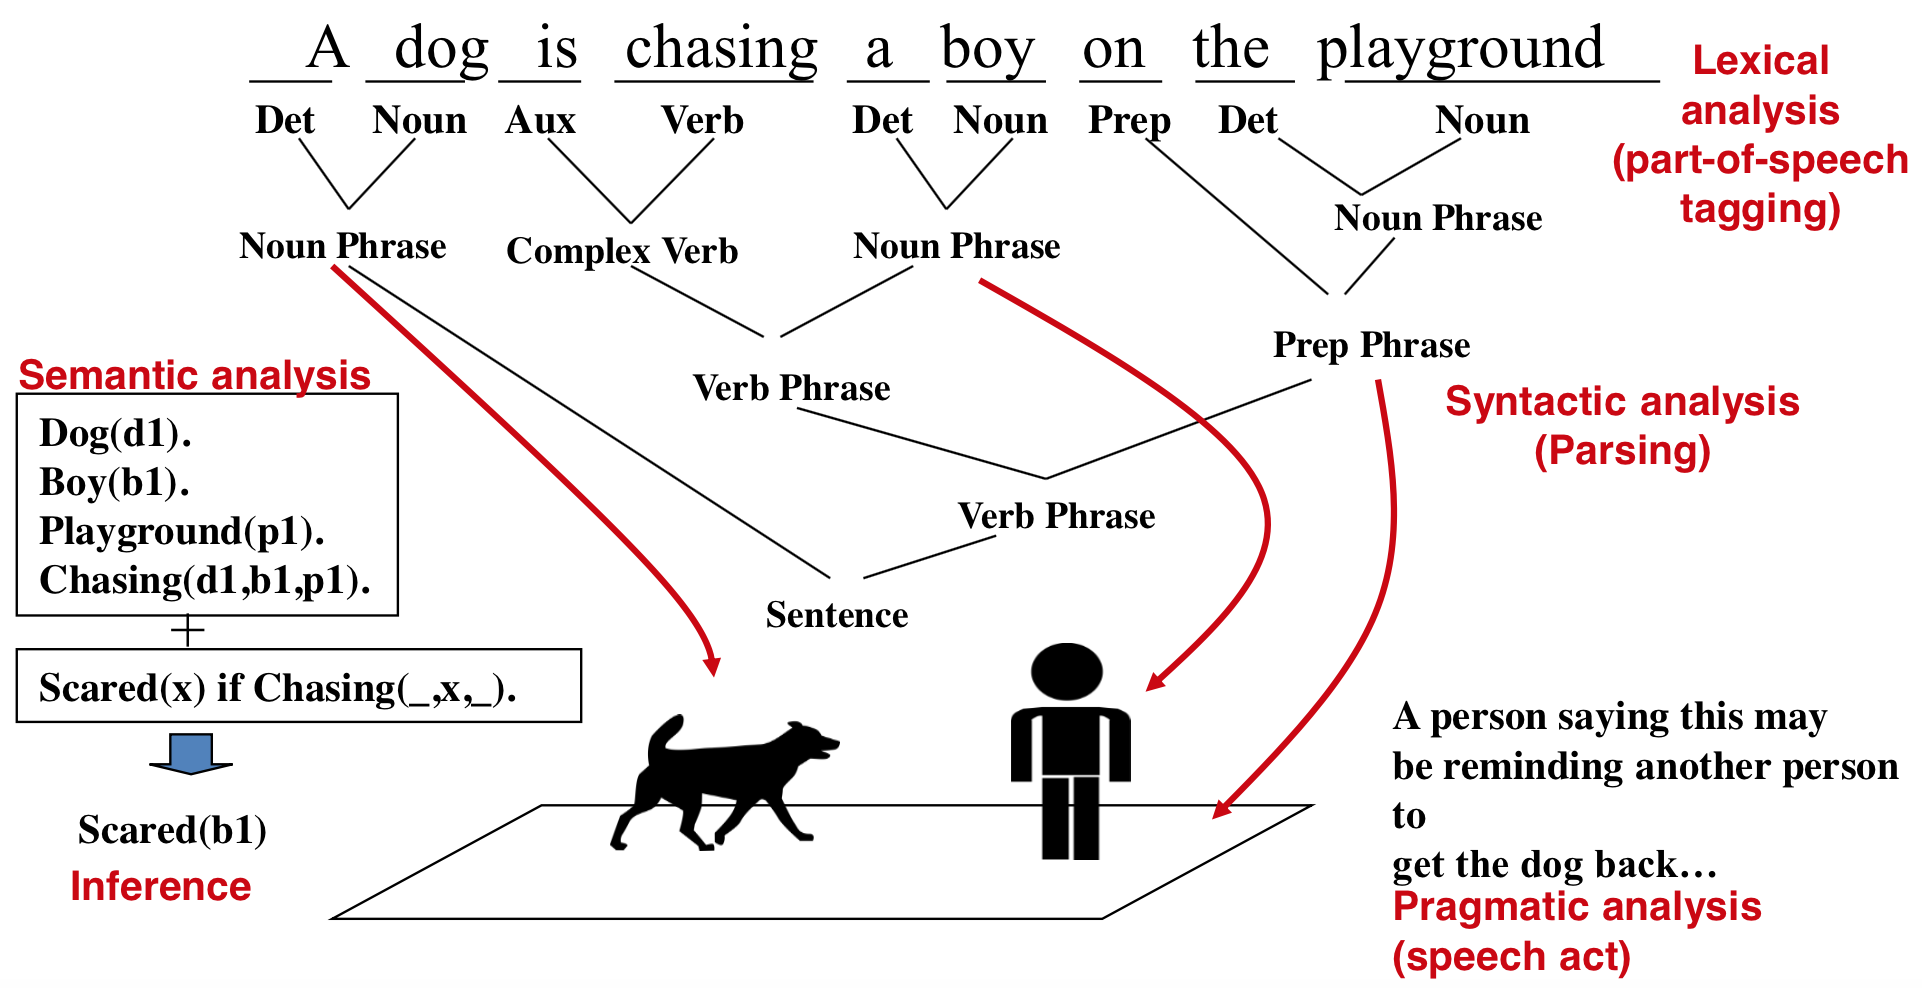
\includegraphics[width=\linewidth]{NLP.png}
\end{figure}

\subsection{The State of the Art}
\begin{figure}[H]
    \centering
    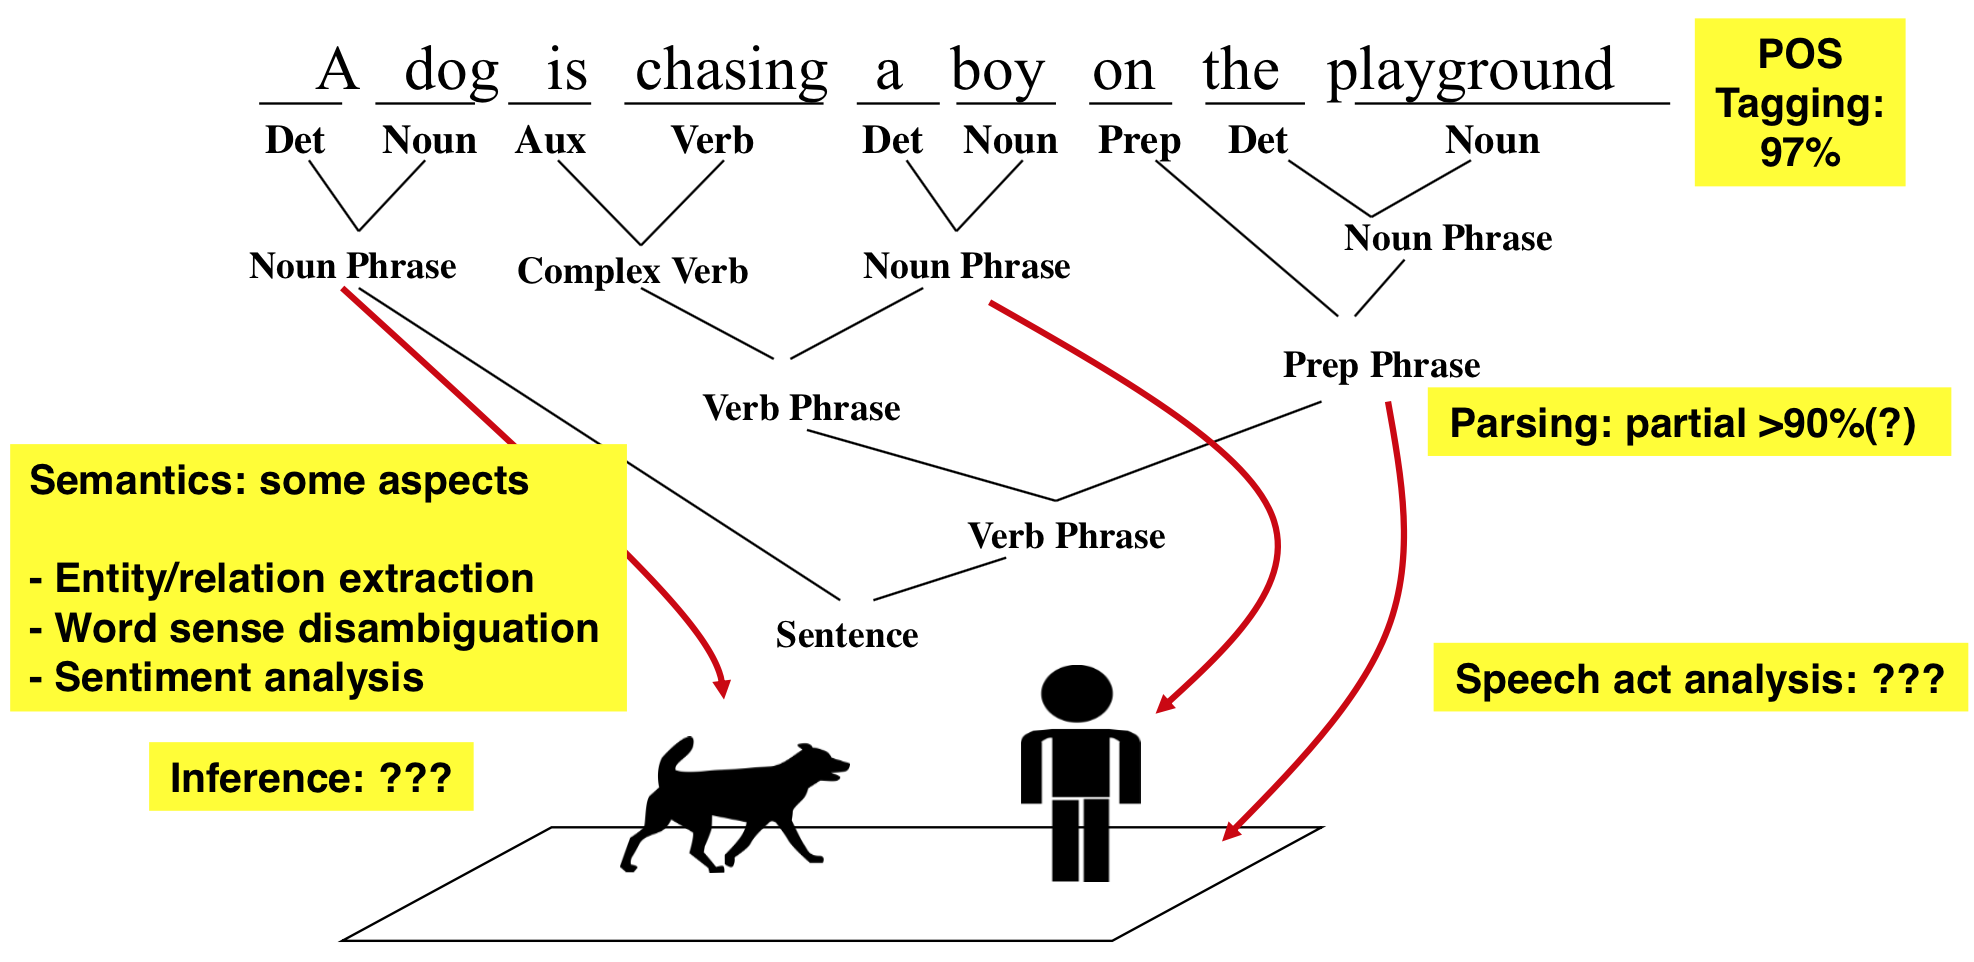
\includegraphics[width=\linewidth]{NLP_state.png}
\end{figure}

\subsection{Recommended reading}
\begin{itemize}
\item Chris Manning and Hinrich Sch{\"u}tze, <<Foundations of Statistical Natural Language Processing>>, MIT Press. Cambridge, MA: May 1999.
\end{itemize}

\section{Lecture 2: Pattern Discovery Basic Concepts}
\subsection{Frequent Itemsets (Patterns)}

X = itemset

\begin{itemize}
\item \textbf{(absolute) support (count) of X:} Frequency or the number of occurrences of an itemset X
\item \textbf{(relative) support, s:} The fraction of transactions that contains X (i.e., the probability that a transaction contains X)
\item An itemset X is \textbf{frequent} if the support of X is no less than a $minsup$ threshold (denoted as $\sigma$)
\end{itemize}

%--
\subsection{Association Rules}
Association rules: $X \to Y (s, c)$:
\begin{itemize}
\item \textbf{Support}, s: The probability that a transaction contains $X \cup Y$
\item \textbf{Confidence}, c: The conditional probability that a transaction containing X also contains Y: 
\begin{equation*}
c = \frac{sup(X \cup Y)}{sup(X)}
\end{equation*}
\end{itemize}

%--
\subsection{Expressing Patterns in Compressed Form}
Solution 1: \textbf{Closed patterns:} \textit{A pattern (itemset) X is closed if X is frequent, and there exists no super-pattern $Y \supset X$, with the same support as X}.\\
    
Closed pattern is a lossless compression of frequent patterns.\\

Solution 2: \textbf{Max-patterns:} \textit{A pattern X is a max-pattern if X is frequent and there exists no frequent super-pattern $Y \supset X$}.\\

Max-pattern is a lossy compression!

%--
\subsection{Recommended readings}
\begin{itemize}
\item R. Agrawal, T. Imielinski, and A. Swami, <<Mining association rules between sets of items in large databases>>, in Proc. of SIGMOD'93
\item R. J. Bayardo, <<Efficiently mining long patterns from databases>>, in Proc. of SIGMOD'98
\item N. Pasquier, Y. Bastide, R. Taouil, and L. Lakhal, <<Discovering frequent closed itemsets
for association rules>>, in Proc. of ICDT'99
\item J. Han, H. Cheng, D. Xin, and X. Yan, <<Frequent Pattern Mining: Current Status and Future Directions>>, Data Mining and Knowledge Discovery, 15(1): 55-86, 2007
\end{itemize}

\section{Lecture 3. Efficient Pattern Mining Methods}
\subsection{The Downward Closure Property of Frequent Patterns}
The downward closure (also called <<Apriori>>) property of frequent patterns: \textbf{Any subset of a frequent itemset must be frequent}. Apriori pruning principle: \textbf{If there is any itemset which is infrequent, its superset should not even be generated!}\\

Scalable mining Methods: Three major approaches
\begin{itemize}
\item Level-wise, join-based approach: Apriori (\ref{apriori})
\item Vertical data format approach: Eclat (\ref{eclat})
\item Frequent pattern projection and growth: FPgrowth (\ref{fpgrowth})
\end{itemize}

%--
\subsection{The Apriori Algorithm}\label{apriori}
\subsubsection{Algorithm pseudocode}
$C_k$: Candidate itemset of size k

$F_k$ : Frequent itemset of size k

TDB = transactional database\\

\begin{algorithm}
\caption{The Apriori Algorithm}
\begin{algorithmic}
\State $k := 1$
\State $F_k :=$ frequent items \Comment{frequent 1-itemset}
\While{$F_k \neq \varnothing$}
    \State $C_{k+1} :=$ candidates generated from $F_k$ \Comment{candidate generation}
    \State Derives $F_{k+1}$ by counting candidates in $C_{k+1}$ with respect to TDB at minsup
    \State $k := k + 1$
\EndWhile
\State \Return $\cup_k F_k$  \Comment{return F\textsubscript{k} generated at each level}
\end{algorithmic}
\end{algorithm}

%--
\subsubsection{How to generate candidates?}

\begin{itemize}
\item Step1: self-joining F\textsubscript{k}
\item Step2: pruning
\end{itemize}


\begin{algorithm}
\caption{Step1: self-joining F\textsubscript{k}}
\begin{algorithmic}
\State insert into C\textsubscript{k}
\State select p.item\textsubscript{1}, p.item\textsubscript{2}, ..., p.item\textsubscript{k-1}, q.item\textsubscript{k-1}
\State from F\textsubscript{k-1} as p, F\textsubscript{k-1} as q
\State where p.item\textsubscript{1}= q.item\textsubscript{1}, ..., p.item\textsubscript{k-2} = q.item\textsubscript{k-2}, p.item\textsubscript{k-1} < q.item\textsubscript{k-1}
\end{algorithmic}
\end{algorithm}

\begin{algorithm}
\caption{Step2: pruning}
\begin{algorithmic}
\ForAll{itemsets c in C\textsubscript{k}}
    \ForAll{(k-1) subsets s of c}
        \If{s is not in F\textsubscript{k-1}}
            \State delete c from C\textsubscript{k}
        \EndIf
    \EndFor
\EndFor
\end{algorithmic}
\end{algorithm}    

%--    
\subsection{Extensions or Improvements of Apriori}
\begin{itemize}
\item Reduce passes of transaction database scans 
    \begin{itemize}
    \item Partitioning
    \item Dynamic itemset counting
    \end{itemize}
\item Shrink the number of candidates
    \begin{itemize}
    \item Hashing
    \item Pruning by support lower bounding
    \item Sampling
    \end{itemize}
\item Exploring special data structures
    \begin{itemize}
    \item Tree projection
    \item H-miner
    \item Hypecube decomposition
    \end{itemize}
\end{itemize}  

%--
\subsubsection{Partitioning}
Theorem: \textit{Any itemset that is potentially frequent in TDB must be frequent in at least one of the partitions of TDB}\\

Method: Scan Database Only Twice:
\begin{itemize}
\item Scan 1: Partition database (how?) and find local frequent patterns
\item Scan 2: Consolidate global frequent patterns (how to?)
\end{itemize}

%--
\subsubsection{Direct Hashing and Pruning (DHP)}
Observation: \textit{A k-itemset whose corresponding hashing bucket count is below the threshold cannot be frequent}

%-- 
\subsection{Vertical Data Format}\label{eclat}
\textbf{ECLAT} - Equivalence Class Transformation

Frequent patterns are derived based on vertical intersections. To accelerate data mining you can use \textbf{diffset}: only keep track of differences of tids.

%--
\subsection{A Pattern Growth Approach}\label{fpgrowth}
\textbf{FP-tree} - frequent pattern tree

\begin{figure}[h!]
    \centering
    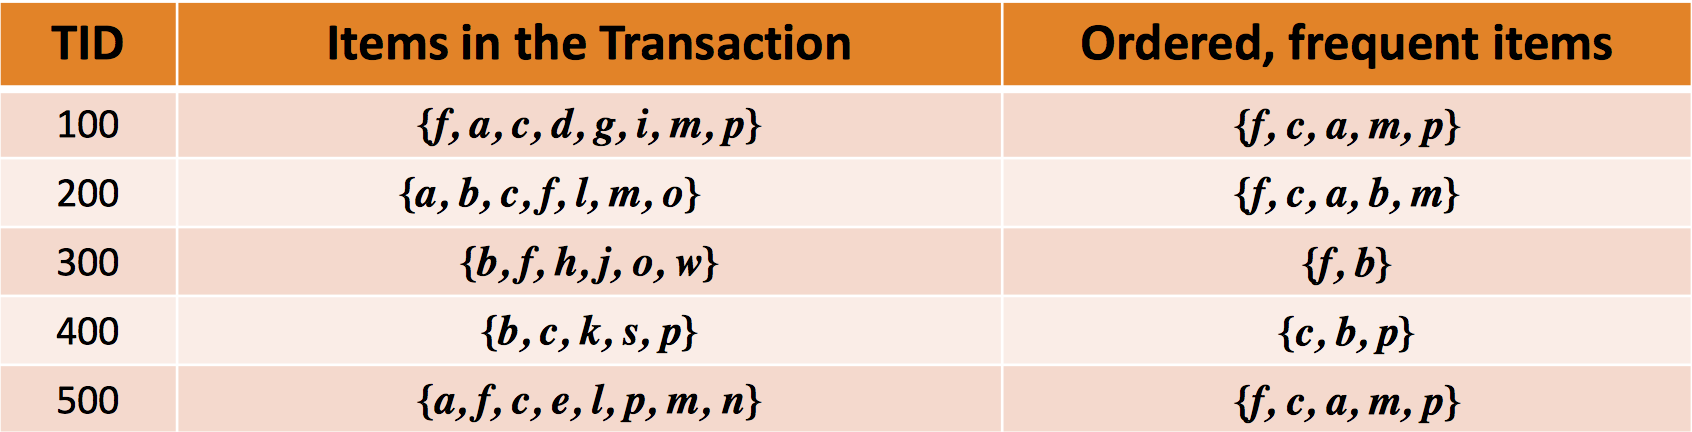
\includegraphics[width=\linewidth]{transactional_db.png}
    \caption{Transational DB}
\end{figure}

\begin{figure}[h!]
    \centering
    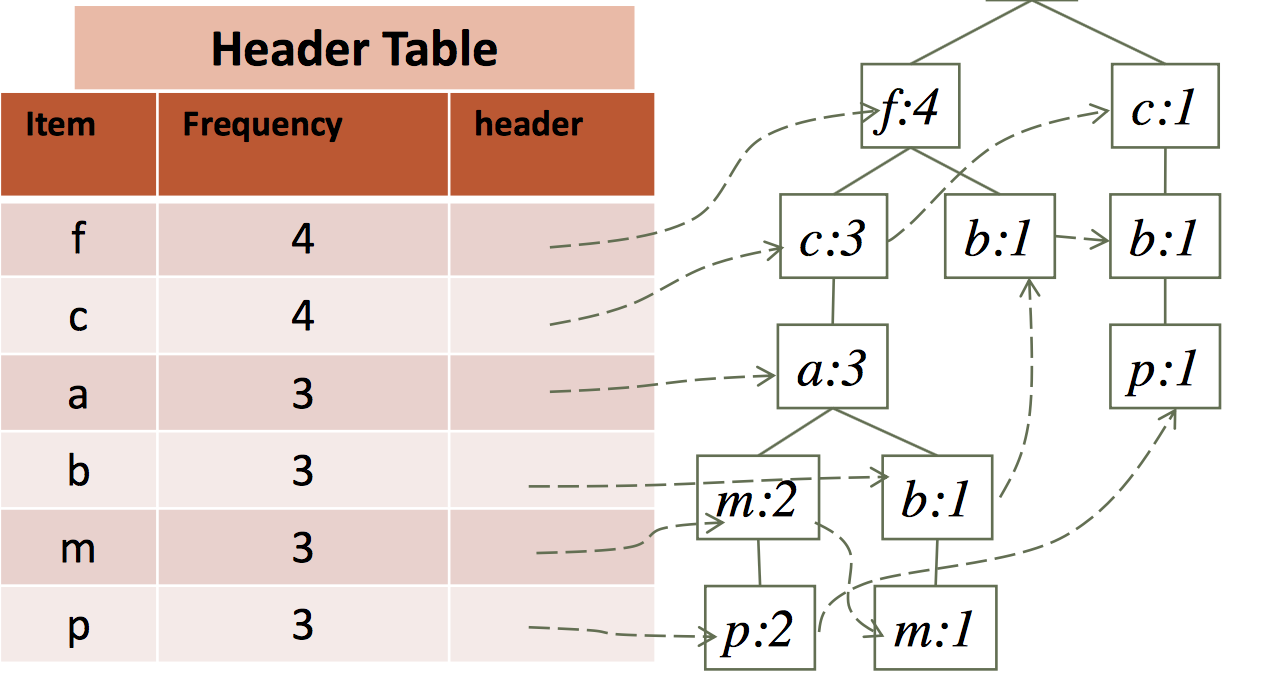
\includegraphics[width=\linewidth]{fptree.png}
    \caption{FP-tree}
\end{figure}

%--
\subsection{CLOSET+: Mining Closed Itemsets by Pattern-Growth}
Itemset merging: \textit{If Y appears in every occurrence of X, then Y
is merged with X}

%--
\subsection{Recommended readings}
\begin{itemize}
\item R. Agrawal and R. Srikant, <<Fast algorithms for mining association rules>>, VLDB'94
\item A. Savasere, E. Omiecinski, and S. Navathe, <<An efficient algorithm for mining association rules in large
databases>>, VLDB'95
\item J. S. Park, M. S. Chen, and P. S. Yu, <<An effective hash-based algorithm for mining association rules>>, SIGMOD'95
\item S. Sarawagi, S. Thomas, and R. Agrawal, <<Integrating association rule mining with relational database systems: Alternatives and implications>>, SIGMOD'98
\item M. J. Zaki, S. Parthasarathy, M. Ogihara, and W. Li, <<Parallel algorithm for discovery of association rules>>, Data Mining and Knowledge Discovery, 1997
\item J. Han, J. Pei, and Y. Yin, <<Mining frequent patterns without candidate generation>>, SIGMOD’00
\item M. J. ZakiandHsiao, <<CHARM: An Efficient Algorithm for Closed Itemset Mining>>, SDM'02
\item J. Wang, J. Han, and J. Pei, <<CLOSET+: Searching for the Best Strategies for Mining Frequent Closed Itemsets>>, KDD'03
\item C. C. Aggarwal, M.A., Bhuiyan, M. A. Hasan, <<Frequent Pattern Mining Algorithms: A Survey>>, in Aggarwal and Han (eds.): Frequent Pattern Mining, Springer, 2014
\end{itemize}
\section{Lecture 4: Pattern Evaluation}

\subsection{Interestingness Measures: Lift and $\mathbf{\chi ^2}$}

\subsubsection{Interestingness Measure: Lift}

\textbf{Lift} - measure of dependent/correlated events:
\begin{equation*}
\mathrm{lift}(B,C) = \frac{c(B \to C)}{s(C)} = \frac{s(B \cup C)}{s(B) \times s(C)}
\end{equation*}

Lift(B, C) may tell how B and C are correlated:
\begin{itemize}
\item $\mathrm{Lift}(B, C) = 1$: B and C are independent
\item $\mathrm{Lift}(B, C) > 1$: positively correlated
\item $\mathrm{Lift}(B, C) < 1$: negatively correlated
\end{itemize}

%--
\subsubsection{Interestingness Measure: $\mathbf{\chi ^2}$}
\begin{equation*}
\chi^2=\sum\frac{(Observed-Expected)^2}{Expected}
\end{equation*}

General rules:
\begin{itemize}
\item $\chi^2 = 0$: independent
\item $\chi^2 > 0$: correlated, either positive or negative, so it needs additional test
\end{itemize}

Too many null transactions may lead to invalid correlation result!

\subsection{Null Invariance Measures}

\begin{gather*}
\mathrm{AllConf}(A, B) = \frac{s(A \cup B)}{\max\{s(A), s(B)\}} \\
\mathrm{Jaccard}(A, B) = \frac{s(A \cup B)}{s(A) + s(B) - s(A \cup B)} \\
\mathrm{Cosine}(A, B) = \frac{s(A \cup B)}{\sqrt{s(A) \times s(B)}} \\
\mathrm{Kulczynsky}(A, B) = \frac{1}{2}\left(\frac{s(A \cup B)}{s(A)} + \frac{s(A \cup B)}{s(B)}\right)\\
\mathrm{MacConf}(A, B)=\max\left\{\frac{s(A)}{s(A \cup B)}, \frac{s(B)}{s(A \cup B)}\right\}
\end{gather*}

\subsection{Imbalance Ratio}
IR (Imbalance Ratio): measure the imbalance of two itemsets A and B in rule implications:
\begin{equation*}
\mathrm{IR}(A, B)=\frac{\abs{s(A)-s(B)}}{s(A) + s(B) - s(A \cup B)}
\end{equation*}

Kulczynski and Imbalance Ratio (IR) together present a clear picture

\subsection{Recommended Readings}
\begin{itemize}
\item C. C. Aggarwal and P. S. Yu. A New Framework for Itemset Generation. PODS’98
\item S. Brin, R. Motwani, and C. Silverstein. Beyond market basket: Generalizing
association rules to correlations. SIGMOD'97
\item M. Klemettinen, H. Mannila, P. Ronkainen, H. Toivonen, and A. I. Verkamo. Finding interesting rules from large sets of discovered association rules. CIKM'94
\item E. Omiecinski. Alternative Interest Measures for Mining Associations. TKDE’03
\item P.-N. Tan, V. Kumar, and J. Srivastava. Selecting the Right Interestingness Measure for
Association Patterns. KDD'02
\item T. Wu, Y. Chen and J. Han, Re-Examination of Interestingness Measures in Pattern Mining: A Unified Framework, Data Mining and Knowledge Discovery, 21(3):371-397, 2010
\end{itemize}
\section{Lecture 4: Mining Diverse Patterns}

\subsection{Mining Multi-Level Associations}

Items often form hierarchies. How to set min-support thresholds? \textbf{Level-reduced min-support}: items at the lower level are expected to have lower support.\\

Efficient mining: \textbf{shared} multi-level mining. Use the lowest min-support to pass down the set of candidates.\\

Redundancy\footnote{Redundancy - избыточность} filtering: some rules may be redundant due to <<ancestor>>\footnote{Ancestor -- предок} relationships between items. A rule is \textbf{redundant} if:
\begin{itemize}
\item its support is close to the <<expected>> value, according to its <<ancestor>> rule
\item it has a similar confidence as its <<ancestor>>.
\end{itemize}\\

It is necessary to have customized min-support settings for different kinds of items: group-based <<individualized>> min-support.

%--
\subsection{Mining Multi-Dimensional Associations}
Rules can be single-dimensional or multi-dimensional:
\begin{itemize}
\item Single-dimentional: 
\begin{equation*}
\mathrm{buys}(X, \text{<<milk>>}) \Rightarrow \mathrm{buys}(X, \text{<<bread>>})
\end{equation*}
\item Inter-dimension association rule: 
\begin{equation*}
\mathrm{age}(X, \text{<<18-25>>}) \wedge \mathrm{occupation}(X, \text{<<student>>}) \Rightarrow \mathrm{buys}(X, \text{<<coke>>})
\end{equation*}
\item Hybrid-dimension association rules: 
\begin{equation*}
\mathrm{age}(X, \text{<<18-25>>}) \wedge \mathrm{buys}(X, \text{<<popcorn>>}) \Rightarrow \mathrm{buys}(X, \text{<<coke>>})
\end{equation*}
\end{itemize}


Attributes can be categorical or numerical

%--    
\subsection{Mining Quantitative Associations}

Methods:
\begin{itemize}
\item Static discretization based on predefined concept hierarchies
\item Dynamic discretization based on data distribution
\item Clustering: distance-based association
\item Deviation analysis
\end{itemize}

%--
\subsection{Mining Negative Correlations}
\begin{itemize}
\item Rare patterns = very low support but interesting
\item Negative patterns = negatively correlated, unlikely to happen together
\end{itemize}

A support-based definition: if itemsets A and B are both frequent but rarely occur together, i.e., $\sup(A \cup B) << \sup (A) \times \sup(B)$ then A and B are negatively correlated.\\

The support-based definition is not null-invariant!\\

A Kulczynski measure-based definition: if itemsets A and B are frequent but $\frac{P(A \mid B) + P(B \mid A)}{2} < \varepsilon$, where $\varepsilon$ is a negative pattern threshold, then A and B are negatively correlated.

%--
\subsection{Mining Compressed Patterns}
\subsubsection{Mining Compressed Patterns}
Pattern distance measure:
\begin{equation*}
Dist(P_1, P_2)=1-\frac{\abs{T(P_1) \cap T(P_2)}}{\abs{T(P_1) \cup T(P_2)}}
\end{equation*}

\textbf{$\mathbf{\delta}$-clustering}. For each pattern P, find all patterns which can be expressed by P and whose distance to P is within $\delta$ ($\delta$-cover). All patterns in the cluster can be represented by P = compressed patterns.\footnote{Method for efficient, direct mining of compressed frequent patterns: Xin et al., VLDB’05.}

\subsubsection{Redundancy-Aware Top-k Patterns}

\begin{figure}[h]
\centering
\subfigure[a set of patterns]{%
  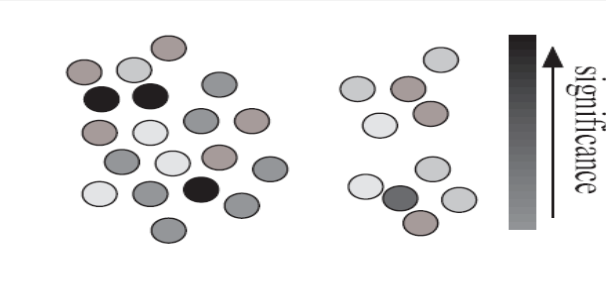
\includegraphics[width=0.32\linewidth, height=0.2\linewidth]{desired_patterns_1.png}
  \label{fig:desired1}}
\quad
\subfigure[redundancy-aware top-k]{%
  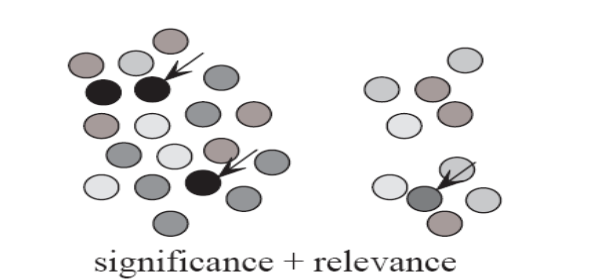
\includegraphics[width=0.32\linewidth, height=0.2\linewidth]{desired_patterns_2.png}
  \label{fig:desired2}}
\subfigure[traditional top-k]{%
  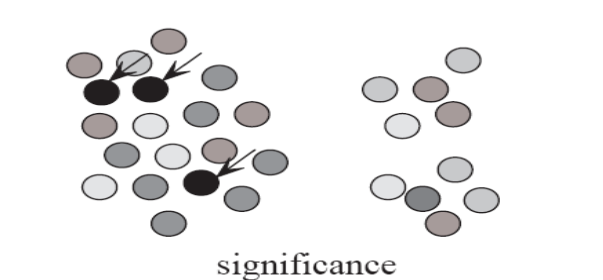
\includegraphics[width=0.32\linewidth, height=0.2\linewidth]{desired_patterns_3.png}
  \label{fig:desired3}}
\quad
\subfigure[summarization]{%
  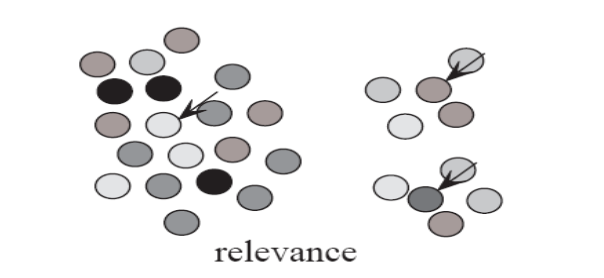
\includegraphics[width=0.32\linewidth, height=0.2\linewidth]{desired_patterns_4.png}
  \label{fig:desired4}}
%
\caption{Desired patterns: high significance \& low redundancy}
\label{fig:desired}
\end{figure}

Use \textbf{MMS (Maximal Marginal Significance)} for measuring the combined significance of a pattern set.\footnote{Xin et al., Extracting Redundancy-Aware Top-K Patterns, KDD’06.}

%--
\subsection{Mining Colossal Patterns}
\subsubsection{Pattern-Fusion}
\textbf{Pattern fusion strategy:} fuse small patterns together in one step to generate new pattern candidates of significant sizes.\\

Subpatterns $\alpha_1$ to $\alpha_k$ cluster tightly around the colossal pattern $\alpha$ by sharing a similar support. Such subpatterns are \textbf{core patterns} of $\alpha$. A colossal pattern can be generated by merging a set of core patterns.

\subsubsection{Robustness of Colossal Patterns}
\begin{definition}
For a frequent pattern $\alpha$, a subpattern $\beta$ is a $\mathbf{\tau}$\textbf{-core pattern} of $\alpha$ if $\beta$ shares a similar support set with $\alpha$, i.e., 
\begin{equation*}
\frac{\abs{D_\alpha}}{\abs{D_\beta}} \geqslant \tau, 0 < \tau \leqslant 1, 
\end{equation*}
where $\tau$ is called the \textbf{core ratio}.
\end{definition}

\begin{definition}
\textbf{$\mathbf{(d, \tau)}$-robustness}\footnote{Robustness - прочность}: a pattern $\alpha$ is $(d, \tau)$-robust if d is the maximum number of items that can be removed from $\alpha$ for the resulting pattern to remain a $\tau$-core pattern of $\alpha$:
\begin{equation*}
d = \max_{\beta}\{\abs{\alpha} - \abs{\beta} \mid \beta \subseteq \alpha\text{, and }\beta\text{ is a }\tau\text{-core pattern of }\alpha\}
\end{equation*}
\end{definition}

For a pattern $\alpha$ let $C_\alpha$ be the set of all its core patterns for a specified $\tau$:
\begin{equation*}
C_\alpha = \{\beta \mid \beta \subseteq \alpha, \frac{\abs{D_\alpha}}{\abs{D_\beta}} \geqslant \tau\}
\end{equation*}

\begin{theorem}
For a $(d, \tau)$-robust pattern $\alpha$:
\begin{equation*}
\abs{C_\alpha} \geqslant 2^d
\end{equation*}
\end{theorem}

\textbf{Robustness of Colossal Patterns}: a colossal pattern tends to have
much more core patterns than small patterns. Such core patterns can be clustered together to form <<dense balls>> based on pattern distance defined by 
\begin{equation*}
Dist(\alpha, \beta)=1-\frac{\abs{D_\alpha \cap D_\beta}}{\abs{D_\alpha \cup D_\beta}}
\end{equation*}

\begin{theorem}
For two patterns $\beta_1, \beta_2 \in C_\alpha$ 
\begin{equation*}
Dist(\beta_1, \beta_2) \leqslant r(\tau)\text{, where }r(\tau)=1-\frac{1}{2/\tau-1}
\end{equation*}
\end{theorem}

\subsubsection{The Pattern-Fusion Algorithm}
\begin{itemize}
\item Initialization (Creating initial pool): Use an existing algorithm to mine all frequent patterns up to a small size, e.g., 3
\item Iteration (Iterative Pattern Fusion):
\begin{itemize}
\item At each iteration, K seed patterns are randomly picked from the current pattern
pool
\item For each seed pattern thus picked, we find all the patterns within a bounding ball centered at the seed pattern
\item All these patterns found are fused together to generate a set of super-patterns
\item All the super-patterns thus generated form a new pool for the next iteration
\end{itemize}
\item Termination: when the current pool contains no more than K patterns at the beginning of an iteration
\end{itemize}

%--
\subsection{Recommended Readings}
\begin{itemize}
\item R. Srikant and R. Agrawal, <<Mining generalized association rules>>, VLDB'95
\item Y. Aumann and Y. Lindell, <<A Statistical Theory for Quantitative Association Rules>>, KDD'99
\item D. Xin, J. Han, X. Yan and H. Cheng, <<On Compressing Frequent Patterns>>, Knowledge and Data Engineering, 60(1): 5-29, 2007
\item D. Xin, H. Cheng, X. Yan, and J. Han, <<Extracting Redundancy-Aware Top-K Patterns>>, KDD'06
\item F. Zhu, X. Yan, J. Han, P. S. Yu, and H. Cheng, <<Mining Colossal Frequent Patterns by Core Pattern Fusion>>, ICDE'07
\item J. Han, H. Cheng, D. Xin, and X. Yan, <<Frequent Pattern Mining: Current Status and Future Directions>>, Data Mining and Knowledge Discovery, 15(1): 55-86, 2007
\end{itemize}
\section{Constraint-Based Pattern Mining}
\subsection{Meta-Rule Guided Mining}
In general, (meta) rules can be in the form of
\begin{equation*}
P_1 \wedge P_2 \wedge ... \wedge P_l \Rightarrow Q_1 \wedge Q_2 \wedge ... \wedge Q_r
\end{equation*}

Method to find meta-rules:
\begin{itemize}
\item Find frequent (l + r) predicates (based on min-support)
\item Push constants deeply when possible into the mining process
\item Also, push min\_conf, min\_correlation, and other measures as early as possible (measures acting as constraints)
\end{itemize}

%--
\subsection{Kinds of Constraints}
\begin{itemize}
\item Pattern space pruning constraints
\begin{itemize}
\item Anti-monotonic: If constraint c is violated, its further mining can be terminated
\item Monotonic: If c is satisfied, no need to check c again
\item Succinct\footnote{Succinct - краткий}: if the constraint c can be enforced by directly manipulating the data
\item Convertible: c can be converted to monotonic or anti-monotonic if items can be properly ordered in processing
\end{itemize}
\item Data space pruning constraints
\begin{itemize}
\item Data succinct: Data space can be pruned at the initial pattern mining process
\item Data anti-monotonic: If a transaction t does not satisfy c, then t can be pruned to reduce data processing effort
\end{itemize}
\end{itemize}

Anti-monotonic constraints have more pruning power than monotonic constraints.

\subsubsection{Pattern space pruning constraints}
Constraint c is \textbf{anti-monotone}: if an itemset S violates constraint \textbf{c}, so does any of its superset. That is, mining on itemset S can be terminated. For example, constraint $\sup(S) \geqslant \sigma$ is anti-monotone.\\

A constraint c is \textbf{monotone}: if an itemset S satisfies the constraint \textbf{c}, so does any of its superset. That is, we do not need to check \textbf{c} in subsequent mining. For example, constraints $\sum(S.price) \geqslant v$ or $\min(S.price) \leqslant v$ are monotone.

\subsubsection{Data space pruning constraints}
A constraint \textbf{c} is \textbf{data anti-monotone}: if a data entry \textbf{t} cannot satisfy a pattern \textbf{p} under constraint \textbf{c}, \textbf{t} cannot satisfy \textbf{p}’s superset either. That's why, data entry \textbf{t} can be pruned.\\

\textbf{Succinctness}: if the constraint \textbf{c} can be enforced by directly manipulating the data.\\

\textbf{Convertible constraints}: convert tough\footnote{Tough - жесткий} constraints into (anti-)monotone by proper ordering of items in transactions. For example, ordering items in value-descending order makes the constraint $avg(S.profit) > 20$ anti-monotone \textit{if the patterns grow in the right order}.

%--
\subsection{Recommended Readings}
\begin{itemize}
\item R. Srikant, Q. Vu, and R. Agrawal, <<Mining association rules with item constraints>>, KDD'97
\item R. Ng, L.V.S. Lakshmanan, J. Han \& A. Pang, Exploratory mining and pruning optimizations of constrained association rules>>, SIGMOD’98
\item G. Grahne, L. Lakshmanan, and X. Wang, <<Efficient mining of constrained correlated sets>>, ICDE'00
\item J. Pei, J. Han, and L. V. S. Lakshmanan, <<Mining Frequent Itemsets with Convertible Constraints>>, ICDE'01
\item J. Pei, J. Han, and W. Wang, <<Mining Sequential Patterns with Constraints in Large Databases>>, CIKM'02
\item F. Bonchi, F. Giannotti, A. Mazzanti, and D. Pedreschi, <<ExAnte: Anticipated Data Reduction in Constrained Pattern Mining>>, PKDD'03
\item F. Zhu, X. Yan, J. Han, and P. S. Yu, <<gPrune: A Constraint Pushing Framework for Graph Pattern Mining>>, PAKDD'07
\end{itemize}

\section{Sequential Pattern Mining}

\subsection{Sequential Pattern}
Sequence $\to$ Element $\to$ Item or Event (items within an element are unordered)

The Apriori property still holds: if a subsequence $s_1$ is infrequent, none of $s_1$’s super-sequences can be frequent.\\

Algorithms:
\begin{itemize}
\item Generalized Sequential Patterns: \textbf{GSP}
\item Vertical format-based mining: \textbf{SPADE}
\item Pattern-growth methods: \textbf{PrefixSpan}
\item Mining closed sequential patterns: \textbf{CloSpan}
\end{itemize}


%--
\subsection{GSP: Apriori- Based Sequential Pattern Mining}

\begin{algorithm}
\caption{GSP}
\begin{algorithmic}
\State k = 1
\Repeat
    \State find length=k frequent sequences
    \State Apriori: remove candidates with sup < min\_sup
    \State length=k frequent sequences $\Rightarrow$ length=(k+1) candidate sequences
    \State k = k + 1
\Until{no frequent sequences or candidates}
\end{algorithmic}
\end{algorithm}


%--
\newpage
\section{Probabilistic Model}

%----------------------------------------
\subsection{Basic Idea of Probabilistic Model}

\begin{itemize}
\item Probabilistic models ranking function: 
\begin{equation*}
f(d, q) = p(R=1 \,\big|\, d,q), \; R \in \{0,1\}
\end{equation*}
\item \textbf{Query Likelihood}: if a user likes document d, how likely would the user enter query q (in order to retrieve d)? 
\item Assumption: a user formulates a query based on an <<imaginary relevant document>>:
\begin{equation*}
p(R=1 \,\big|\, d,q) \approx p(q \,\big|\, d,R=1)
\end{equation*}
\item Basic idea based on user clicks (R=1):
\begin{equation*}
f(q, d) = p(R=1 \,\big|\, d,q) = \frac{count(q, d, R=1)}{count(q,d)}
\end{equation*}
\item How to compute $p(q \,|\, d)$? How to compute probability of
text in general? $\to$ \textbf{Language Model}
\end{itemize}


%----------------------------------------
\subsection{Language Model}
The term language model (LM) refers to a probabilistic model of text (i.e., it defines a probability distribution over sequences of words). 

Uses of a Language Model:
\begin{itemize}
\item Representing topics
\item Discovering word associations
\end{itemize}


%----------------------------------------
\subsection{The Simplest Language Model: Unigram LM}
Unigram Language Model = word distribution
\begin{itemize}
\item Generate text by generating each word \textbf{independently} 
\item Thus, $p(w_1, w_2 \dots w_n) = p(w_1)p(w_2) \dots p(w_n)$
\item Parameters: $\{p(w_i)\}: p(w_1) + \ldots + p(w_N) = 1$ (N is vocabulary size)
\item Text = sample drawn according to this \textbf{word distribution}
\end{itemize}

Maximum Likelihood (ML) Estimator:
\begin{equation*}
p(w \,\big|\, \theta) = p(w \,\big|\, d) = \frac{c(w, d)}{|d|}
\end{equation*}
\begin{itemize}
\item $\theta$ - document language model
\item $c(w, d)$ - count on word $w$ in document $d$
\item $|d|$ - length of document $d$
\end{itemize}

%----------------------------------------
\subsection{Recommended reading}
\begin{itemize}
\item Chris Manning and Hinrich Sch{\"u}tze, <<Foundations of Statistical Natural Language Processing>>, MIT Press. Cambridge, MA: May 1999.
\item  Rosenfeld, R., <<Two decades of statistical language modeling: where do we go from here?>>, Proceedings of the IEEE , vol.88, no.8, pp.1270,1278, Aug. 2000
\end{itemize}

%----------------------------------------
\subsection{Ranking based on Query Likelihood}

\begin{itemize}
\item Query: $q = w_1 w_2 \dots w_n$
\item Vocabulary of the language of the documents: $V = \{ w_1, \dots ,w_{|V|} \}$
\item $c(w, q)$ - count of word $w$ in query $q$
\end{itemize}

How likely would we observe this query from this document model?
\begin{equation*}
p(q \:\big|\: d) = p(w_1 \:\big|\: d) \times \dots \times p(w_n \:\big|\: d)
\end{equation*}

Retrieval problem $\to$ estimation of $p(w_i \,\big|\, d)$
\begin{equation*}
f(q, d) = \log p(q \,\big|\, d) = \sum_{i=1}^{n} \log p(w_i \,\big|\, d) = \sum_{w \in V} c(w, q) \cdot \log p(w \,\big|\, d)
\end{equation*}

%----------------------------------------
\subsection{How to Estimate $p(w \big| d)$}
Smoothing of $p(w \big| d)$ is necessary for query likelihood:
\begin{figure}[H]
    \centering
    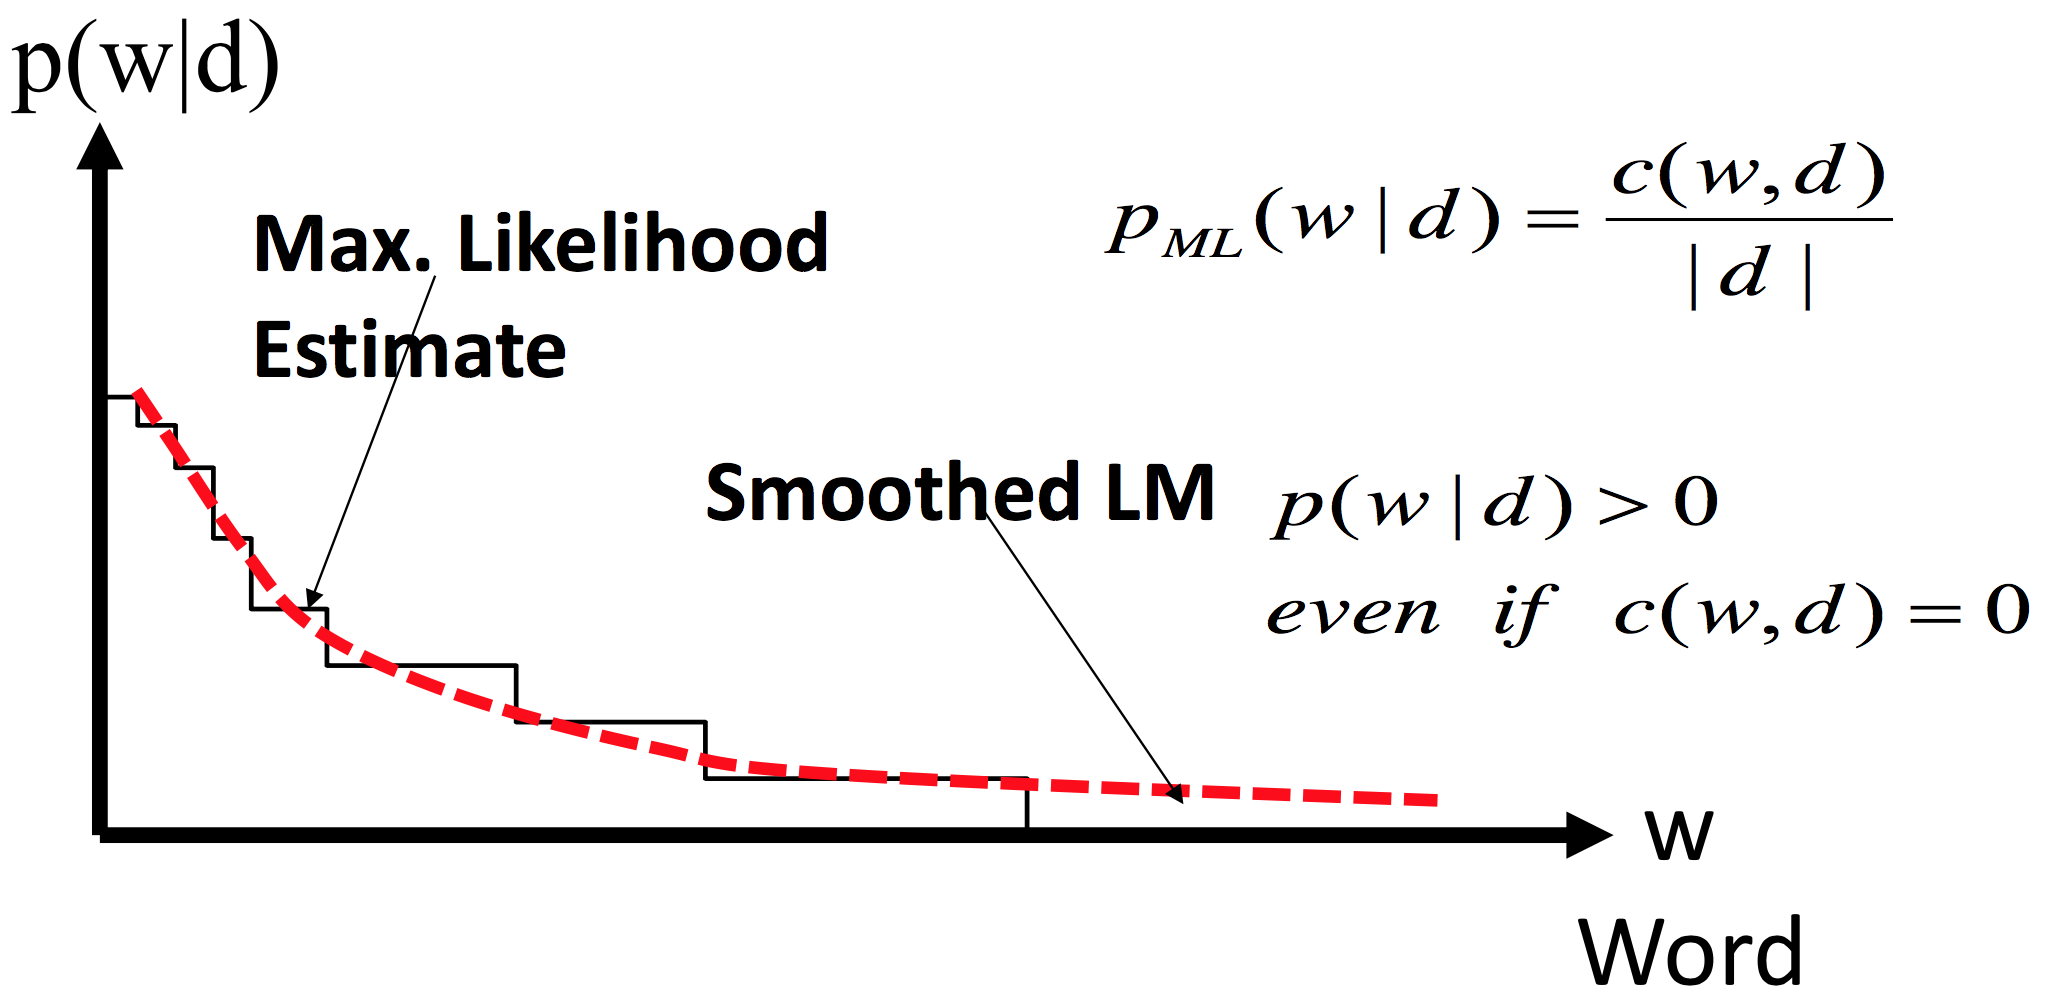
\includegraphics[width=0.7\linewidth]{smoothed_lm.png}
\end{figure}

Key Question: what probability should be assigned to an unseen word? Let the probability of an unseen word be proportional to its probability given by a reference LM. One possibility: Reference LM = Collection LM:
\begin{figure}[H]
    \centering
    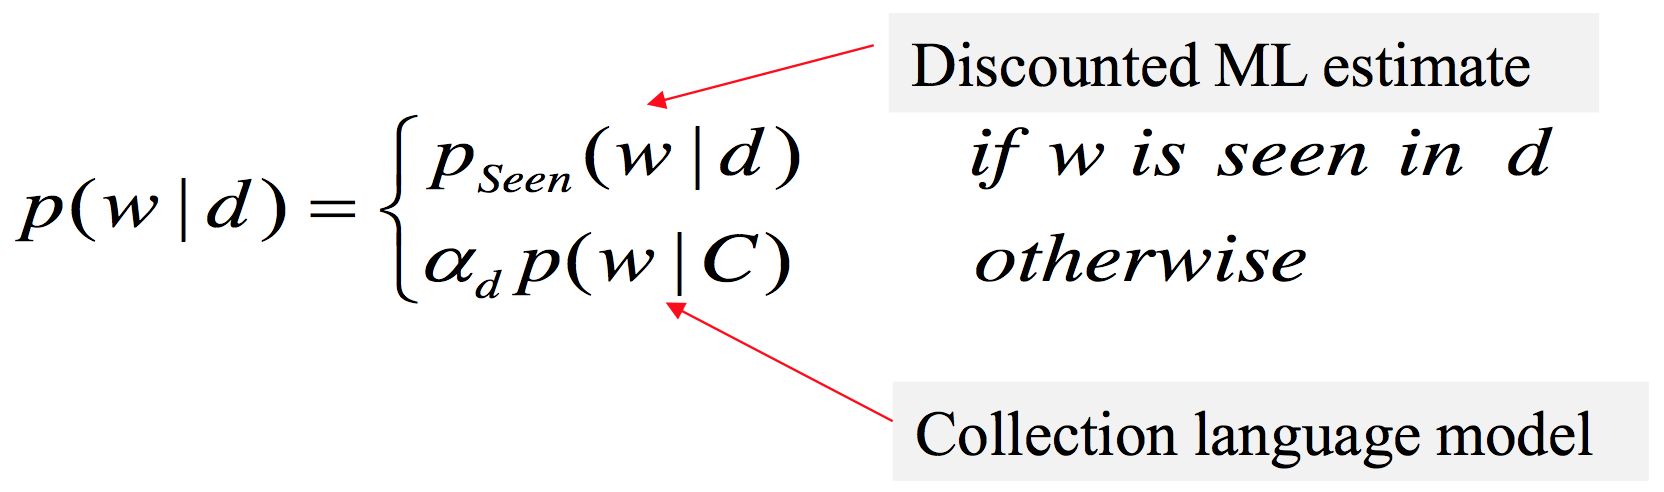
\includegraphics[width=0.6\linewidth]{probability_lm.png}
\end{figure}

%----------------------------------------
\subsection{Rewriting the Ranking Function with Smoothing}
\begin{figure}[H]
    \centering
    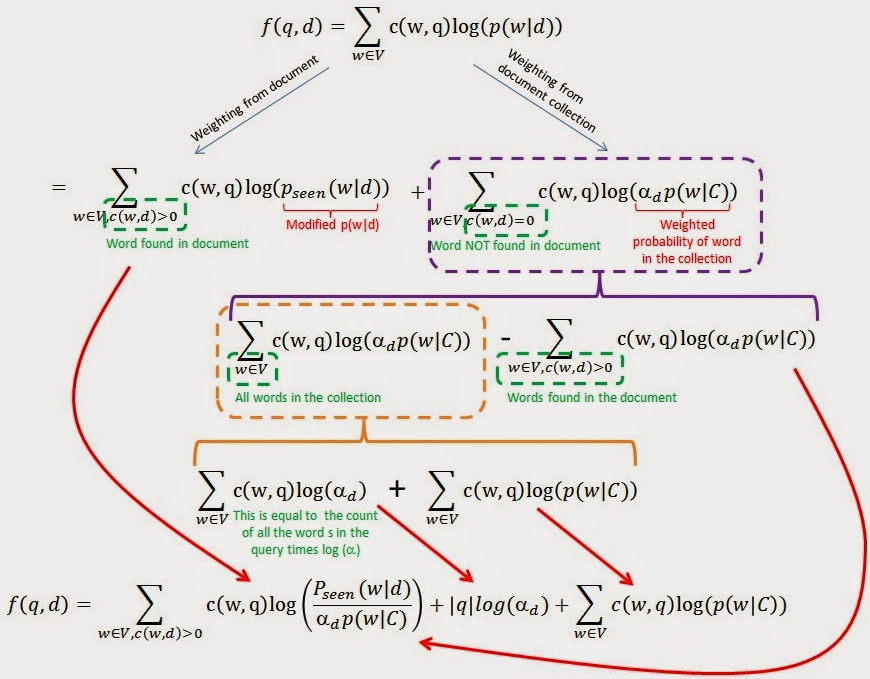
\includegraphics[width=\linewidth]{ranking_smoothing.png}
\end{figure}

%----------------------------------------
\subsection{Benefit of Rewriting}

Smoothing with $p(w \big| d)$ leads to a general ranking formula for query likelihood with TF- IDF weighting and document length normalization:
\begin{figure}[H]
    \centering
    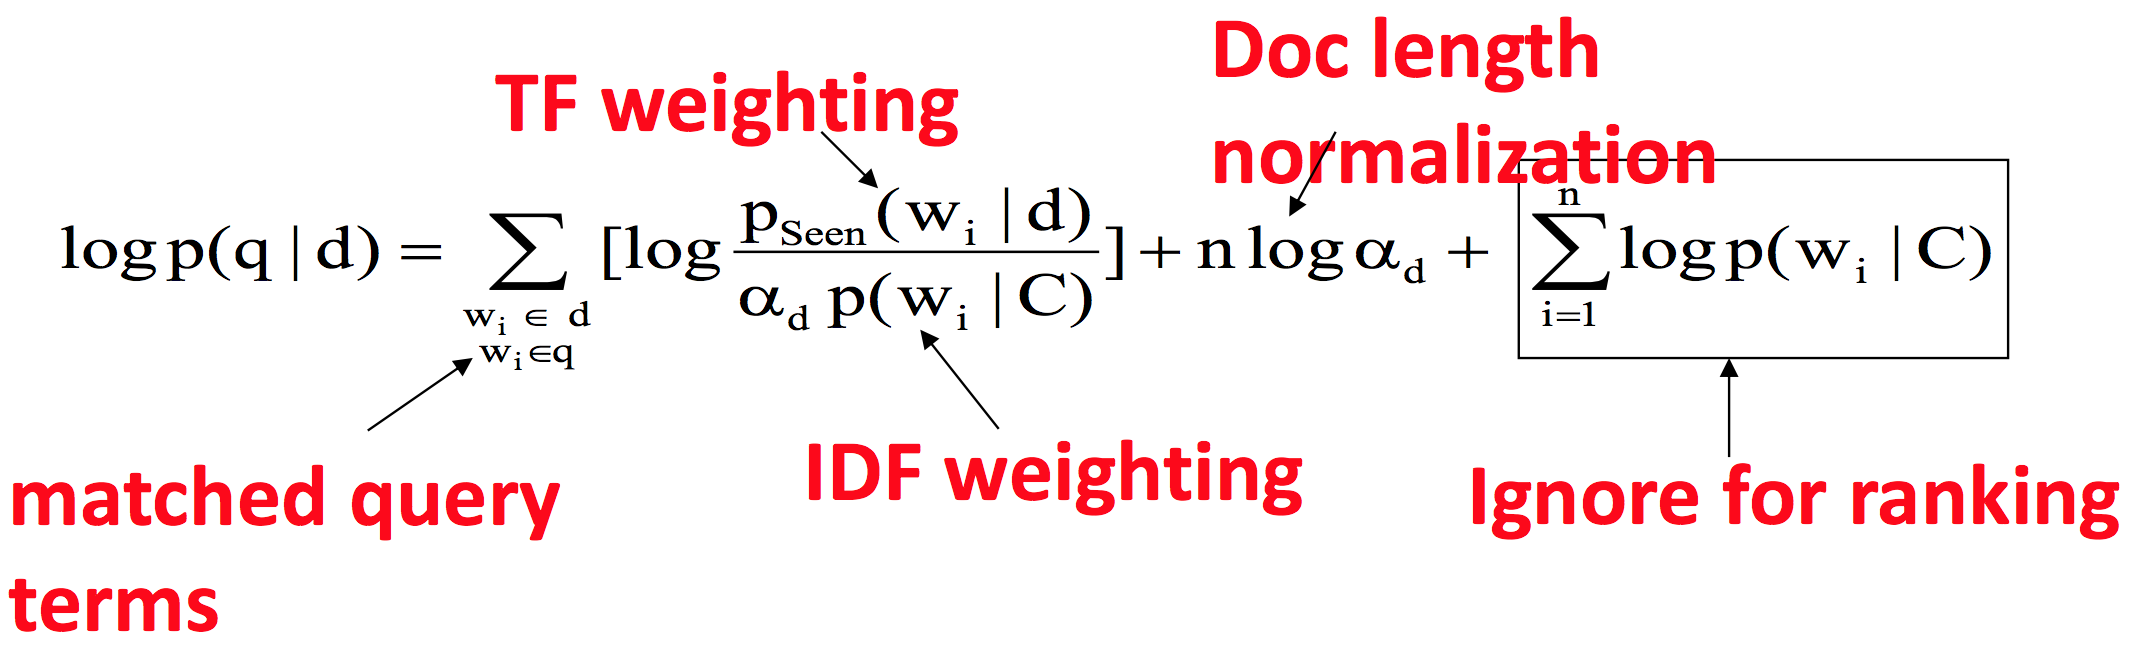
\includegraphics[width=0.8\linewidth]{ranking_smoothed.png}
\end{figure}

%----------------------------------------
\subsection{Smoothing Methods}
\begin{equation*}
f(q, d) = \sum_{w_i \in d, w_i \in q} c(w_i, q) \log \frac{p_{seen}(w_i \,\big|\, d)}{\alpha_d \, p(w_i \,\big|\, C)} + n \log \alpha_d
\end{equation*}

\subsubsection{Jelinek-Mercer Smoothing}
Jelinek-Mercer: Fixed coefficient linear interpolation
\begin{equation*}
p_{seen}(w \,\big|\, d) = (1-\lambda) \, \dfrac{c(w, d)}{|d|} + \lambda \, p(w \,\big|\, C), \quad \alpha_d = \lambda, \quad \lambda \in [0, 1]
\end{equation*}

Ranking Function:
\begin{equation*}
f_{JM}(q, d) = \sum_{w \in d, w \in q} c(w, q) \log \left( 1 + \frac{1-\lambda}{\lambda} \frac{c(w, d)}{|d| \, p(w \,\big|\, C)} \right)
\end{equation*}

\subsubsection{Dirichlet Prior (Bayesian) Smoothing}
Dirichlet Prior: Adding pseudo counts; adaptive interpolation
\begin{equation*}
p_{seen}(w \,\big|\, d) = \dfrac{c(w, d) + \mu \, p(w \,\big|\, C)}{|d| + \mu} = \dfrac{|d|}{|d| + \mu}\cdot\dfrac{c(w,d)}{|d|} + \dfrac{\mu}{|d| + \mu}\cdot p(w \,\big|\, C)
\end{equation*}

\begin{equation*}
\alpha_d = \frac{\mu}{|d| + \mu}, \quad \mu \in [0, +\infty)
\end{equation*}

Ranking Function:
\begin{equation*}
f_{DIR}(q, d) = \sum_{w \in d, w \in q} c(w, q) \log \left( 1 + \frac{c(w, d)}{\mu \, p(w \,\big|\, C)} \right) + n\,\log\frac{\mu}{\mu + |d|}
\end{equation*}

%----------------------------------------
\subsection{Summary of Query Likelihood Probabilistic Model}
\begin{itemize}
\item Effective ranking functions obtained using pure probabilistic modeling

\begin{itemize}
\item Assumption 1: $Relevance(q,d) = p(R=1 \,\big|\, q,d) \approx p(q \,\big|\, d,R=1) \approx p(q \,\big|\, d)$
\item Assumption 2: Query words are generated independently
\item Assumption 3: Smoothing with $p(w \,\big|\, C)$
\item Assumption 4: JM or Dirichlet prior smoothing
\end{itemize}

\item Less heuristic compared with VSM
\item Many extensions have been made [Zhai 08]
\end{itemize}

%----------------------------------------
\subsection{Recommended reading}
\begin{itemize}
\item ChengXiang Zhai, \href{http://www.morganclaypool.com/doi/abs/10.2200/S00158ED1V01Y200811HLT001}{<<Statistical Language Models for Information Retrieval>> (Synthesis Lectures Series on Human Language Technologies)}, Morgan \& Claypool Publishers, 2008.
\end{itemize}


\section{Lecture 9. Pattern-Based Classification}

\subsection{Classification: Basic Concepts}

\begin{figure}[H]
    \centering
    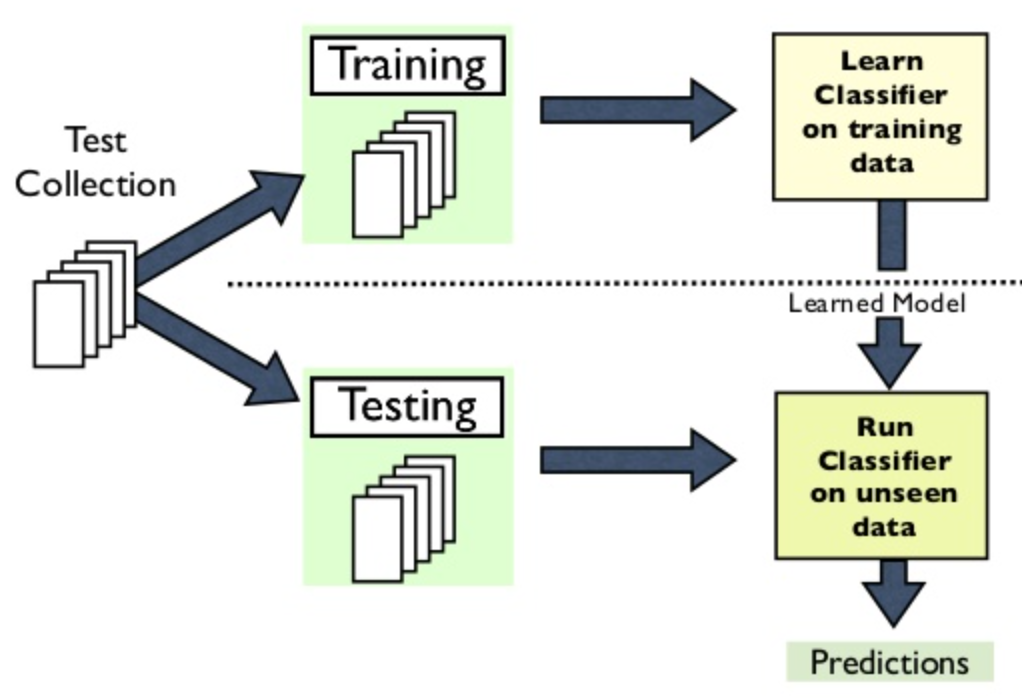
\includegraphics[width=0.7\linewidth]{classification.png}
    \caption{Classification}
\end{figure}

Typical Classification Methods:
\begin{itemize}
\item Support Vector Machines
\item Decision Tree
\item Neural Network
\item Bayesian Network
\end{itemize}

%--
\subsection{Pattern-based classification methods}
\begin{itemize}
\item CBA [Liu, Hsu \& Ma, KDD’98]: Use high-conf., high-support class association rules to build classifiers
\item Emerging patterns [Dong \& Li, KDD’99]: Patterns whose support changes significantly between the two classes
\item CMAR [Li, Han \& Pei, ICDM’01]: Multiple rules in prediction
\item CPAR [Yin \& Han, SDM’03]: Beam search on multiple prediction rules
\item RCBT [Cong et al., SIGMOD’05]: Build classifier based on mining top-k covering rule groups with row enumeration (for high-dimensional data)
\item Lazy classifier [Veloso, Meira \& Zaki, ICDM’06]: For a test t, project training data D on t, mine rules from $D_t$ , predict on the best rule
\item Discriminative pattern-based classification [Cheng et al., ICDE’07]
\end{itemize}

%--
\subsection{CBA: Classification Based on Associations}
\begin{itemize}
\item Mine high-confidence, high-support class association rules
\item LHS: conjunctions of attribute-value pairs); RHS: class labels\\
$p_1 \wedge p_2 ... \wedge p_l \to \left[A_{class-label} = C\right]$
\item Rank rules in descending order of confidence and support
\item Classification: Apply the first rule that matches a test case; otherwise apply the default rule
\end{itemize}

%--
\subsection{CMAR: Classification Based on Multiple Association Rules}
Rule pruning whenever a rule is inserted into the tree:
\begin{itemize}
\item Given two rules, $R_1$ and $R_2$, if the antecedent\footnote{Antecedent - предшественник} of $R_1$ is more general than that of $R_2$ and $conf(R_1) \geqslant conf(R_2)$, then prune $R_2$
\item Prunes rules for which the rule antecedent and class label are not positively correlated, based on the $\chi^2$ test of statistical significance
\end{itemize}

Classification based on generated/pruned rules:
\begin{itemize}
\item If only one rule satisfies tuple X, assign the class label of the rule \item If a ruleset S satisfies X
\begin{itemize}
\item Divide S into groups according to class labels
\item Use a weighted $\chi^2$ measure to find the strongest group of rules, based on the statistical correlation of rules within a group 
\item Assign X the class label of the strongest group
\end{itemize}
\end{itemize}

%--
\subsection{Discriminative Pattern-Based Classification}
\textbf{Principle:} Mining discriminative frequent patterns as high-quality
features and then apply any classifier.

Framework (\textbf{PatClass}):
\begin{itemize}
\item Feature construction by \textbf{frequent itemset mining}
\item Feature selection (e.g., using \textbf{Maximal Marginal Relevance (MMR)})
\begin{itemize}
\item Select \textbf{discriminative features} (i.e., that are relevant but minimally similar to the previously selected ones)
\item Remove redundant or closely correlated features 
\end{itemize}
\item Model learning: apply a general classifier, such as SVM or C4.5, to build a classification model
\end{itemize}

\subsubsection{On the Power of Discriminative Patterns}
K-itemsets are often more informative than single features (1-itemsets) in classification. Computation on real datasets shows: the discriminative power of k-itemsets (for $k > 1$ but often $\leqslant 10$) is higher than that of single features.\\

Computation on real datasets shows: pattern frequency (but not too frequent) is strongly tied with the discriminative power (information gain). Information gain upper bound monotonically increases with pattern frequency.

\begin{figure}[H]
\centering
\subfigure[IG vs. Pattern Length]{%
  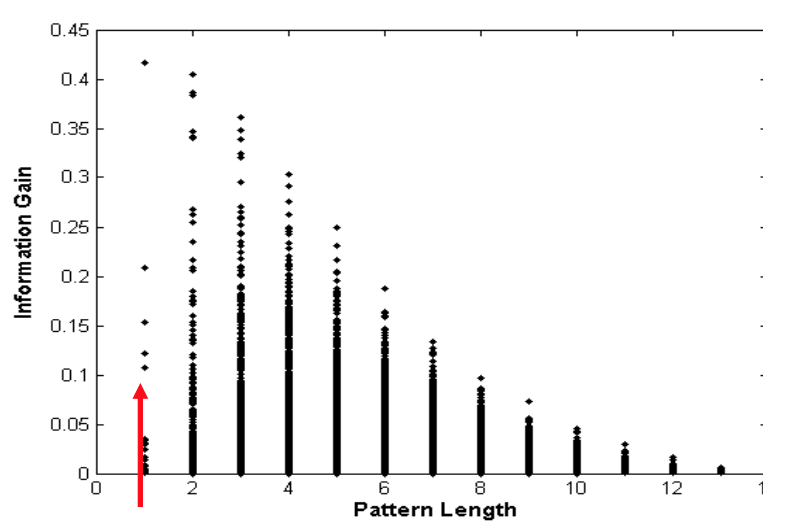
\includegraphics[width=0.42\linewidth, height=0.2\linewidth]{ig_len.png}
  \label{fig:ig1}}
\quad
\subfigure[IG vs. Frequency]{%
  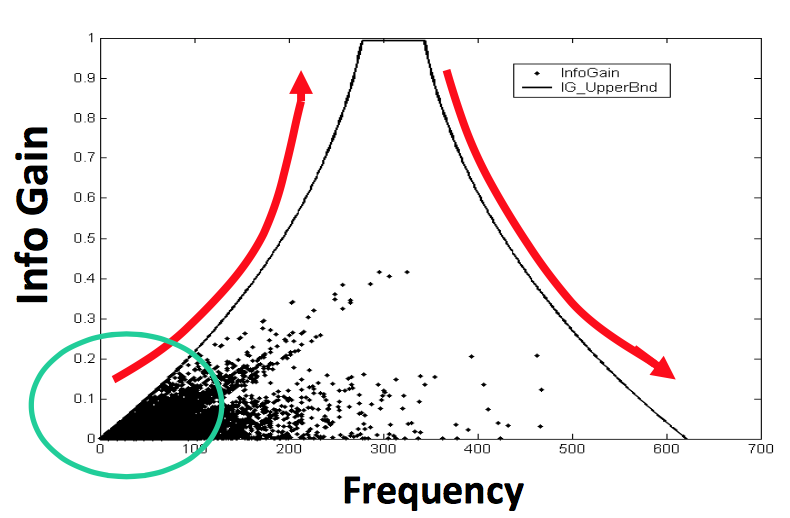
\includegraphics[width=0.42\linewidth, height=0.2\linewidth]{ig_freq.png}
  \label{fig:ig2}}
\caption{Information Gain}
\label{fig:ig}
\end{figure}

Information gain formula:
\begin{gather*}
IG (C \mid X) = H (C) - H (C \mid X)\text{, where }\\
H(C) = -\sum^{m}_{i=1}p_i \log_2(p_i)\text{ - entropy of given data}\\
H(C \mid X) = \sum_j P(X=x_j) H(Y \mid X=x_j)\text{ - conditional entropy of study focus}
\end{gather*}

%--
\subsection{DDPMine: Direct Mining of Discriminative Patterns}
General methodology:
\begin{itemize}
\item Input: A set of training instances D and a set of features F
\item Iteratively perform feature selection based on the \textbf{<<sequential coverage>>} paradigm
\begin{itemize}
\item Select the feature fi with the highest discriminative power
\item Remove instances Di from D covered by the selected feature fi
\end{itemize}
\end{itemize}

Implementation:
\begin{itemize}
\item Integration of \textbf{branch-and-bound search} with FP-growth mining
\item Iteratively eliminate training instances and \textbf{progressively shrink the FP-tree}
\end{itemize}

\subsubsection{Branch-and-Bound Search}
\begin{itemize}
\item The discriminative power (information gain) of a low frequency pattern is upper bounded by a small value
\item During FPGrowth mining we record the most discriminative itemset discovered so far and its information gain value $g_{best}$
\begin{itemize}
\item Before constructing a conditional FP-tree, we first estimate the upper bound of information gain based on the conditional DB
\item If the upper bound value $\leqslant g_{best}$, skip this conditional FP-tree and its subsequent trees
\end{itemize}
\end{itemize}



%--
\subsection{Recommended Readings}
\begin{itemize}
\item H. Cheng, X. Yan, J. Han \& C.-W. Hsu, Discriminative Frequent Pattern Analysis for Effective Classification, ICDE'07
\item H. Cheng, X. Yan, J. Han \& P. S. Yu, Direct Discriminative Pattern Mining for Effective Classification, ICDE’08
\item G. Cong, K. Tan, A. Tung \& X. Xu. Mining Top-k Covering Rule Groups for Gene Expression Data, SIGMOD’05
\item M. Deshpande, M. Kuramochi, N. Wale \& G. Karypis. Frequent Substructure-based Approaches for Classifying Chemical Compounds, TKDE’05
\item G. Dong \& J. Li. Efficient Mining of Emerging Patterns: Discovering Trends and Differences, KDD’99
\item W. Fan, K. Zhang, H. Cheng, J. Gao, X. Yan, J. Han, P. S. Yu \& O. Verscheure. Direct Mining of
Discriminative and Essential Graphical and Itemset Features via Model-based Search Tree, KDD’08
\item W. Li, J. Han \& J. Pei. CMAR: Accurate and Efficient Classification based on Multiple Class-association Rules, ICDM’01
\item B. Liu, W. Hsu \& Y. Ma. Integrating Classification and Association Rule Mining, KDD’98
\item J. Wang and G. Karypis. HARMONY: Efficiently Mining the Best Rules for Classification, SDM’05
\item X. Yin \& J. Han. CPAR: Classification Based on Predictive Association Rules, SDM’03
\end{itemize}


%\newpage
\section{Web Search}

\subsection{Web Search: Challenges \& Opportunities}
Web search is one of the most important applications of text retrieval.
\begin{itemize}
\item Challenges
\begin{itemize}
\item Scalability (the size of the Web, completeness of coverage, many user queries) $to$ Parallel indexing \& searching (MapReduce)
\item Low quality information and spams $to$ Spam detection \& Robust ranking
\item Dynamics of the Web (new pages are constantly created, some pages may be updated)
\end{itemize}

\item Opportunities
\begin{itemize}
\item many additional heuristics (e.g., link information, layout) can be leveraged to improve search accuracy $to$ Link analysis \& multi-feature ranking
\end{itemize}
\end{itemize}


%---------------------------------------------
\subsection{Basic Search Engine Technologies}
\begin{figure}[H]
    \centering
    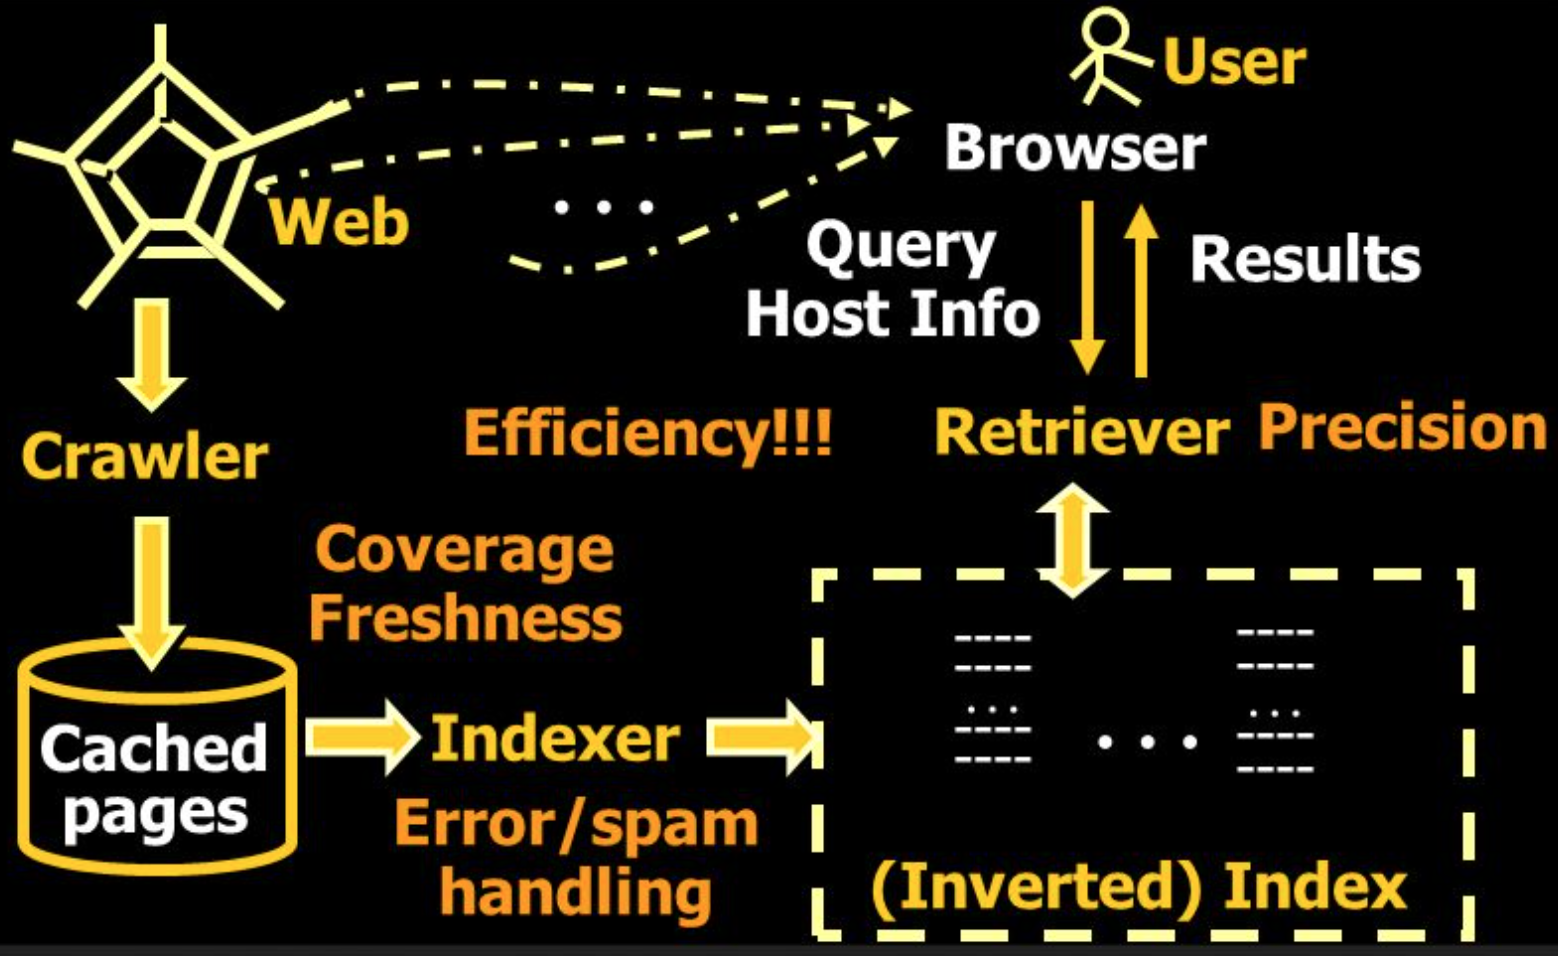
\includegraphics[width=0.9\linewidth]{search_engine.png}
\end{figure}

%---------------------------------------------
\subsection{Crawler/Spider/Robot}

\begin{itemize}
\item Building a <<toy crawler>> is easy
\begin{itemize}
\item Start with a set of “seed pages” in a priority queue
\item Fetch pages from the web
\item Parse fetched pages for hyperlinks; add them to the queue 
\item Follow the hyperlinks in the queue
\end{itemize}

\item A real crawler is much more complicated... 
\begin{itemize}
\item Robustness (server failure, trap, etc.)
\item Crawling courtesy (server load balance, robot exclusion, etc.) 
\item Handling file types (images, PDF files, etc.)
\item URL extensions (cgi script, internal references, etc.)
\item Recognize redundant pages (identical and duplicates)
\item Discover <<hidden>> URLs (e.g., truncating a long URL )
\end{itemize}
\end{itemize}

%--------------
\subsubsection{Major Crawling Strategies}
\begin{itemize}
\item Breadth-First\footnote{\textbf{Breadth-first search (BFS)} is an algorithm for traversing or searching tree or graph data structures. It starts at the tree root (or some arbitrary node of a graph, sometimes referred to as a <<search key>>) and explores the neighbor nodes first, before moving to the next level neighbors.} is common (balance server load)
\item Parallel crawling is natural

\item Variation: focused crawling
\begin{itemize}
\item Targeting at a subset of pages (e.g., all pages about <<automobiles>>) 
\item Typically given a query
\end{itemize}

\item How to find new pages (they may not linked to an old page!)

\item Incremental/repeated crawling
\begin{itemize}
\item Need to minimize resource overhead
\item Can learn from the past experience (updated daily vs. monthly)
\item Target at : 1) frequently updated pages; 2) frequently accessed pages
\end{itemize}
\end{itemize}

%---------------------------------------------
\subsection{Web Index}

Standard IR techniques are the basis, but insufficient – they lack scalability and efficiency. \\

Google’s contributions:
\begin{itemize}
\item Google File System (GFS): distributed file system
\item MapReduce: Software framework for parallel computation 
\item Hadoop: Open source implementation of MapReduce
\end{itemize}

%--------------
\subsubsection{GFS Architecture}
\begin{figure}[H]
    \centering
    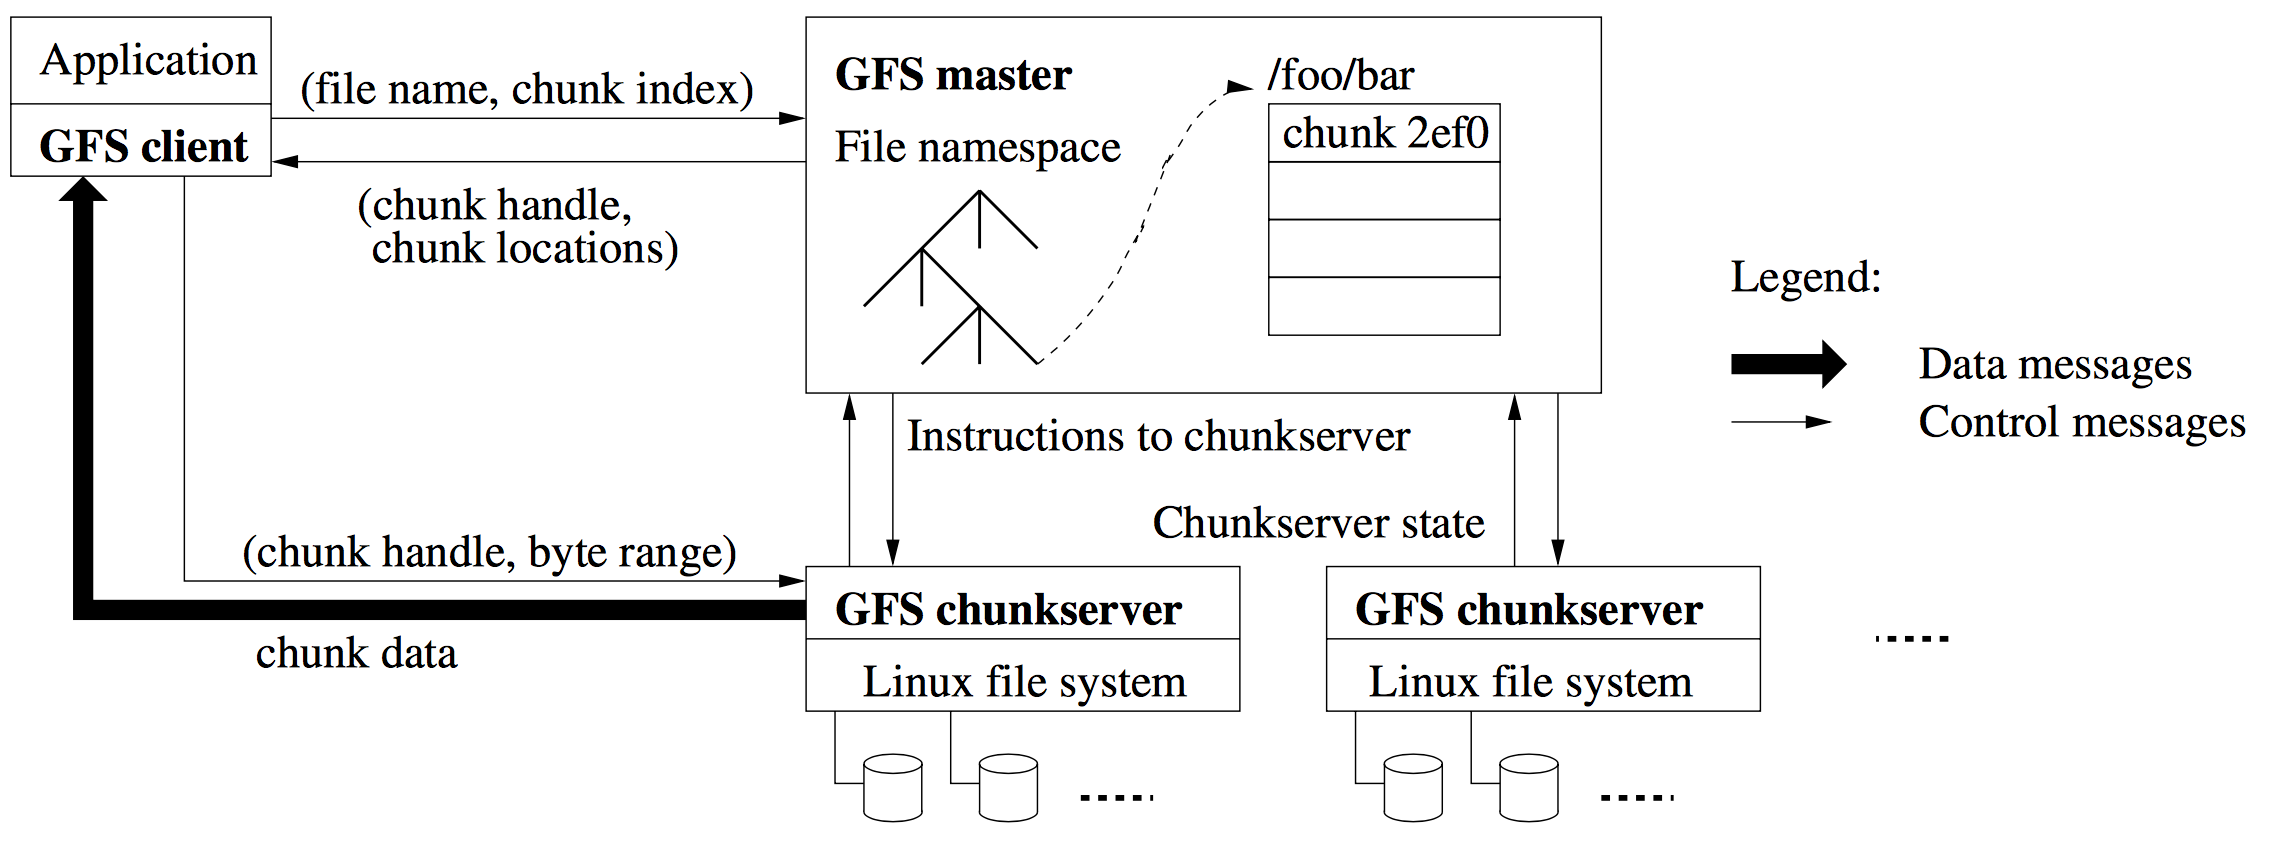
\includegraphics[width=\linewidth]{GFS.png}
\end{figure}

%--------------
\subsubsection{MapReduce: A Framework for Parallel Programming}
\begin{itemize}
\item Minimize effort of programmer for simple parallel processing tasks
\begin{itemize}
\item Features
\item Hide many low-level details (network, storage) 
\item Built-in fault tolerance
\item Automatic load balancing
\end{itemize}
\end{itemize}


%--------------
\subsubsection{MapReduce: Computation Pipeline}
\begin{figure}[H]
    \centering
    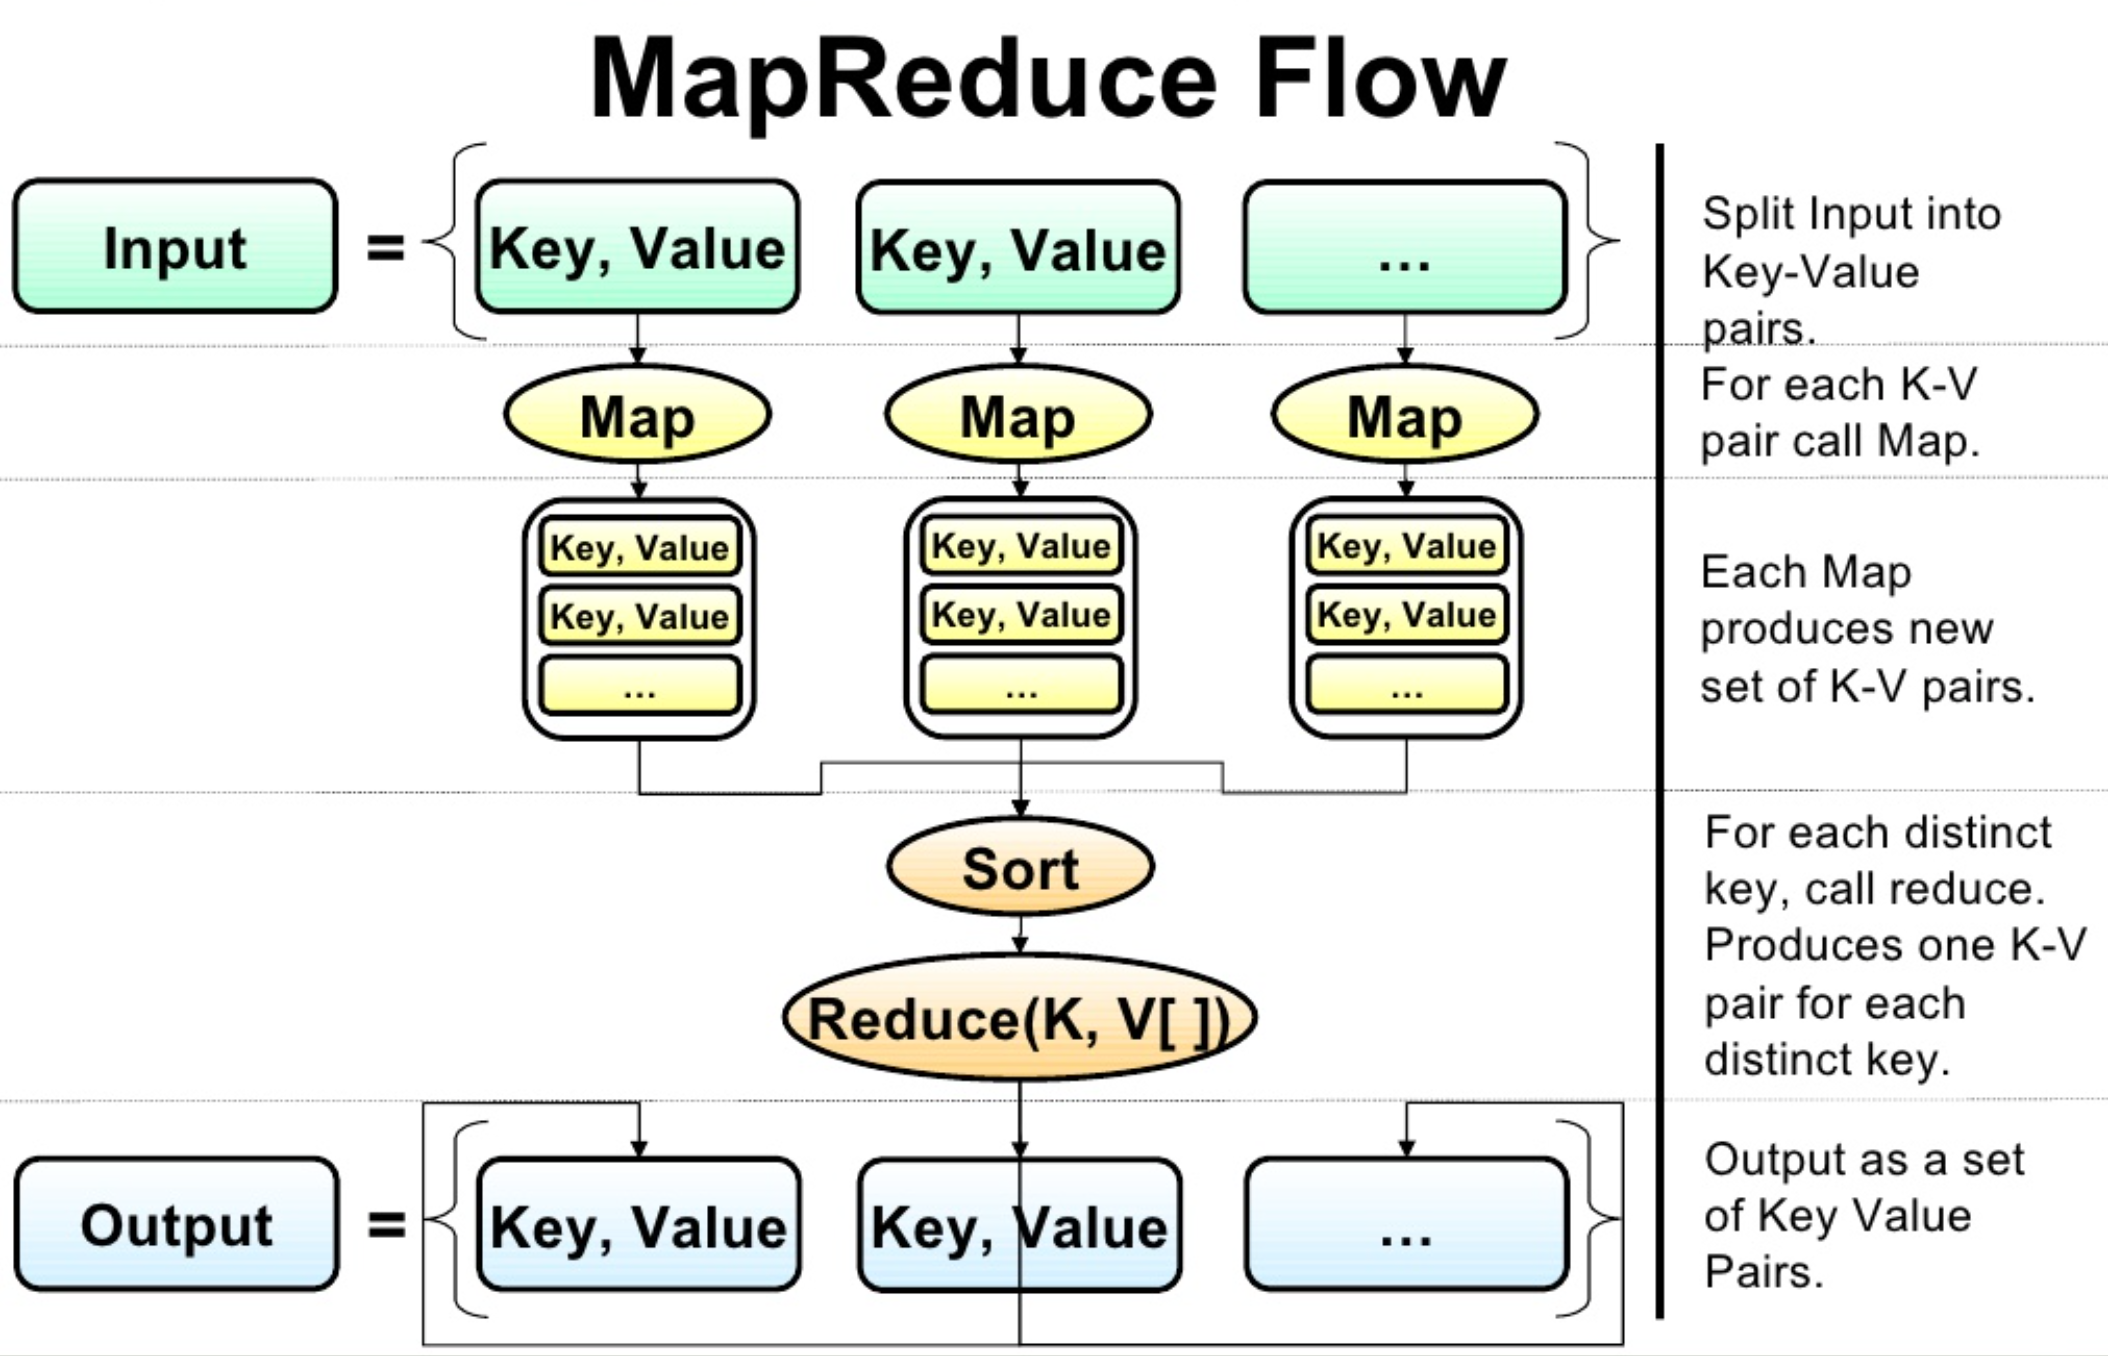
\includegraphics[width=\linewidth]{map_reduce.png}
\end{figure}


%--------------
\subsubsection{Inverted Indexing with MapReduce}

\begin{figure}[H]
    \centering
    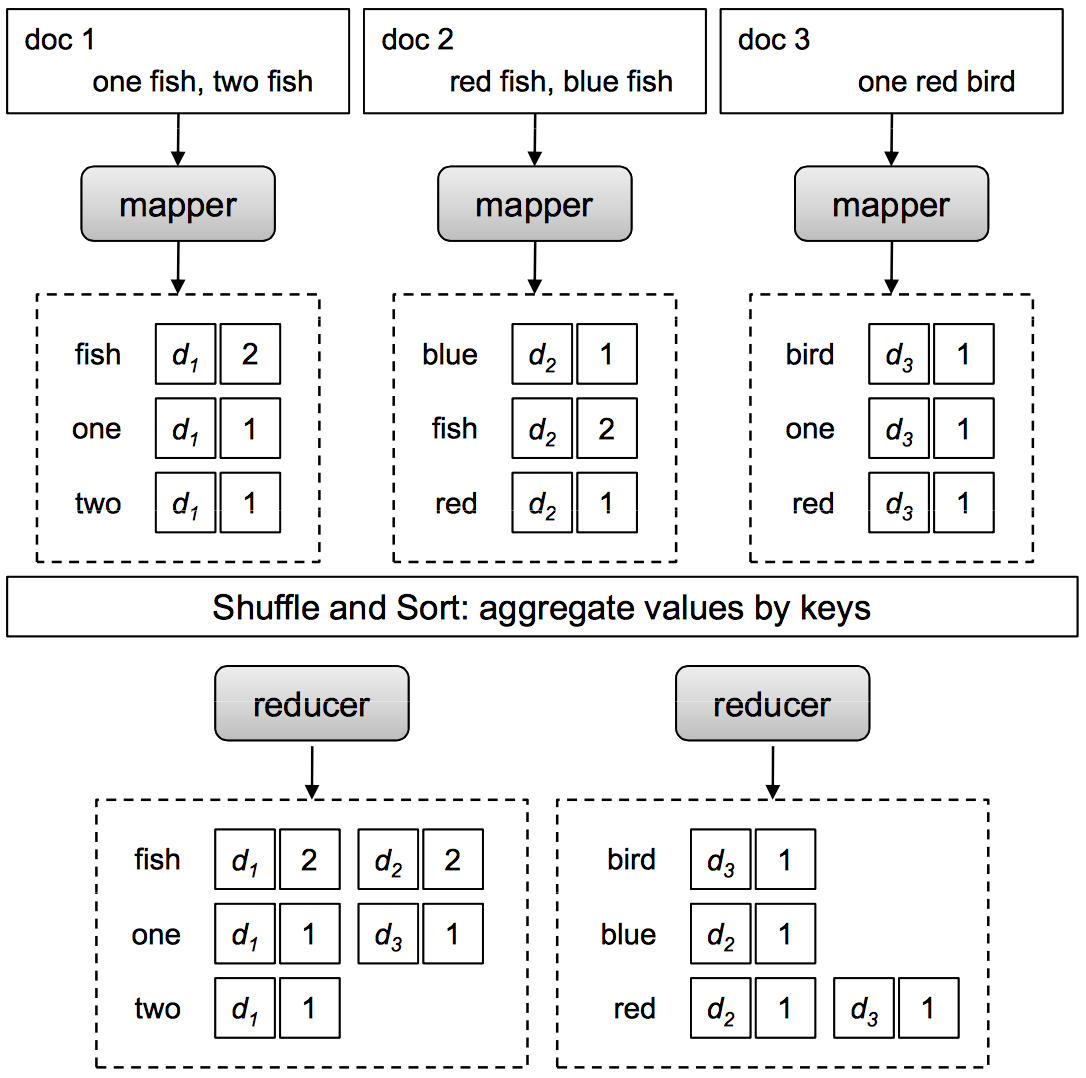
\includegraphics[width=0.8\linewidth]{mapreduce_inverted_index.png}
\end{figure}


\begin{algorithm}
\caption{Pseudo-code of the baseline inverted indexing algorithm in MapReduce}
\begin{algorithmic}
\State \textbf{class} Mapper
    \Procedure {Map}{docid $n$, doc $d$}
        \State $H \gets$ new AssociativeArray
        \ForAll {term $t \in$ doc $d$} 
            \State $H\{T\} \gets H\{T\}+1$
        \EndFor
        \ForAll {term $t \in H$}
            \State Emit(term $t$, posting $\langle n, H\{t\} \rangle$)
        \EndFor
    \EndProcedure  
    
    \State
\State \textbf{class} Reducer
    \Procedure{Reduce}{term $t$, postings $[\langle n_1, f_1 \rangle, \langle n_2, f_2 \rangle \dots]$}
        \State $P \gets$ new List
        \ForAll {posting $\langle a,f \rangle \in$ postings $[\langle n_1, f_1 \rangle, \langle n_2, f_2 \rangle \dots]$}
            \State Append($P$, $\langle a,f \rangle$) 
        \EndFor
        \State Sort($P$)
        \State Emit(term $t$, postings $P$)         
    \EndProcedure           
\end{algorithmic}
\end{algorithm}



%---------------------------------------------
\subsection{Link Analysis}

\subsubsection{Ranking Algorithms for Web Search}
\begin{itemize}
\item Standard IR models apply but aren’t sufficient 
\begin{itemize}
\item Different information needs (search for a particular web page instead of text information)
\item Documents have additional information (links, layout)
\item Information quality varies a lot
\end{itemize}

\item Major extensions
\begin{itemize}
\item Exploiting links to improve scoring
\item Exploiting clickthroughs for massive implicit feedback
\item In general, rely on machine learning to combine all kinds of features
\end{itemize}
\end{itemize}


%--------------
\subsubsection{Exploiting Inter-Document Links}

Description of a link (\textbf{<<anchor text>>}) is a summary and a query example for a target document.\\

An \textbf{authority} is a web page containing valuable information with respect to a specific subject. A \textbf{hub} is a web page not actually authoritative in the information it holds, but contains useful links toward an authoritative page – basically, advertising the authoritative web page.

\begin{figure}[H]
    \centering
    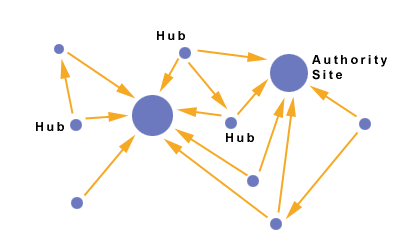
\includegraphics[width=0.8\linewidth]{hubs_and_authorities.png}
\end{figure}


%--------------
\subsubsection{PageRank: Capturing Page <<Popularity>>}
\begin{itemize}
\item Intuitions
\begin{itemize}
\item Links are like citations in literature
\item A page that is cited often can be expected to be more useful in general
\end{itemize}

\item PageRank is essentially <<citation counting>>, but improves over simple counting
\begin{itemize}
\item Consider <<indirect citations>> (being cited by a highly cited paper counts a lot...)
\item Smoothing of citations (every page is assumed to have a non-zero pseudo citation count)
\end{itemize}

\item PageRank can also be interpreted as random surfing (thus capturing popularity)
\end{itemize}


%--------------
\subsubsection{The PageRank Algorithm}

\begin{multicols}{2}
\begin{figure}[H]
    \centering
    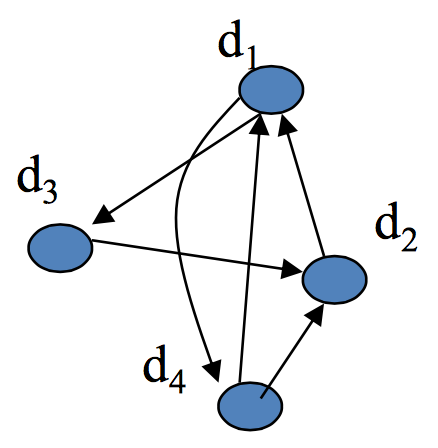
\includegraphics[width=0.7\linewidth]{page_rank_example.png}
\end{figure}


Transition matrix:
\begin{equation*}
M = 
\begin{pmatrix}
 0  &  0  & 1/2 & 1/2 \\
 1  &  0  &  0  &  0 \\
 0  &  1  &  0  &  0 \\
1/2 & 1/2 &  0  &  0 
\end{pmatrix}
\end{equation*}

$M_{ij}$ - probability of going from $d_i$ to $d_j$:

\begin{equation*}
\forall i: \sum_{j=1}^{N} M_{ij} = 1
\end{equation*}
\end{multicols}

\vspace{5mm}
<<Equilibrium Equation>>:
\begin{equation*}
p_{t+1}(d_j) = (1-\alpha) \sum_{i=1}^{N}M_{ij}\:p_t(d_i) + \alpha \sum_{i=1}^{N}\frac{1}{N}\:p_t(d_i),
\end{equation*}
where 
\begin{itemize}
\item $N$ - number of pages
\item $p_t(d_i)$ - probability of visiting page $d_i$ at time $t$
\item $\alpha$ - probability of jumping to a random page
\end{itemize}

\vspace{5mm}
For a converged\footnote{Converge - сходиться} state we can drop the time index:
\begin{equation*}
p(d_j) = \sum_{i=1}^{N} \left[ \frac{1}{N} \: \alpha + (1-\alpha) M_{ij} \right ] p(d_i) 
\end{equation*}
and come to this equation:
\begin{equation*}
\vec{p} = \Big(\alpha I + (1-\alpha) M \Big)^T \; \vec{p}, \text{ where } I_{ij} = \frac{1}{N},
\end{equation*}
which can be solved with an iterative algorithm starting with initial value $p(d)=1/N$.  

%--------------
\subsubsection{PageRank in Practice}
\begin{itemize}
\item Computation can be quite efficient since M is usually sparse
\item Normalization doesn’t affect ranking, leading to some variants of the formula

\item The zero-outlink problem: $p(d_i)$’s don’t sum to 1
\begin{itemize}
\item One possible solution = page-specific damping factor\footnote{Damping factor - коэффициент затухания}
($\alpha=1.0$ for a page with no outlink)
\end{itemize}
\item Many extensions (e.g., topic-specific PageRank)
\item Many other applications (e.g., social network analysis)
\end{itemize}


%--------------
\subsubsection{HITS: Capturing Authorities \& Hubs}
\begin{itemize}
\item Intuitions
\begin{itemize}
\item Pages that are widely cited are good authorities 
\item Pages that cite many other pages are good hubs
\end{itemize}

\item The key idea of HITS (Hypertext-Induced Topic Search) 
\begin{itemize}
\item Good authorities are cited by good hubs
\item Good hubs point to good authorities
\item Iterative reinforcement...
\end{itemize}

\item Many applications in graph/network analysis
\end{itemize}


%--------------
\subsubsection{The HITS Algorithm}

\begin{multicols}{2}
\begin{figure}[H]
    \centering
    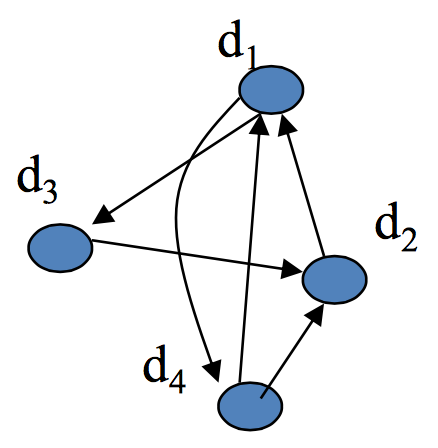
\includegraphics[width=0.7\linewidth]{page_rank_example.png}
\end{figure}


<<Adjacency matrix>>\footnote{<<Adjacency matrix>> $\approx$ матрица связей (<<соседства>>)}:
\begin{equation*}
A = 
\begin{pmatrix}
 0  &  0  &  1  &  1 \\
 1  &  0  &  0  &  0 \\
 0  &  1  &  0  &  0 \\
 1  &  1  &  0  &  0 
\end{pmatrix}
\end{equation*}


Algorithm:
\begin{itemize}
\item Initial values: $a(d_i)=h(d_i)=1$
\item Iteration:
\begin{equation*}
\begin{cases}
h(d_i) = \sum_{d_j \in OUT(d_i)} a(d_j) \\
a(d_i) = \sum_{d_j \in IN(d_i)} h(d_j)
\end{cases}
\end{equation*}
\item Iteration in matrix form:
\begin{equation*}
\begin{cases}
\vec{h} = A\,\vec{a} = AA^T\,\vec{h} \\
\vec{a} = A^T\,\vec{h} = A^TA\,\vec{a}
\end{cases}
\end{equation*}
\item Normalize: $\sum_i a(d_i)^2 = \sum_i h(d_i)^2 = 1$
\end{itemize}

\end{multicols}


%---------------------------------------------
\subsection{Learning to Rank}
%--------------
\subsubsection{How Can We Combine Many Features?}
\begin{itemize}
\item Given a query-doc pair $(Q,D)$, define various kinds of features
$X_i(Q ,D)$
\item Examples of feature:
\begin{itemize}
\item the number of overlapping terms, 
\item BM25 score of $Q$ and $D$, 
\item $p(Q \,\big|\, D)$, 
\item PageRank of $D$, 
\item $p(Q \,\big|\, D_i)$, where $D_i$ may be anchor text or big font text, 
\item <<does the URL contain ‘~’?>> 
\item etc.
\end{itemize}
\item Hypothesize $p(R=1 \,\big|\, Q, D) = s\big( X_1(Q,D), \dots ,X_n(Q,D), \lambda \big)$, where $\lambda$ is a set of parameters
\item Learn $\lambda$ by fitting function s with training data, i.e., 3-tuples like $(D, Q, 1)$ ($D$ is relevant to $Q$) or $(D,Q,0)$ ($D$ is non-relevant to $Q$)
\end{itemize}

%--------------
\subsubsection{Regression-Based Approaches}

Logistic Regression: 
\begin{itemize}
\item $X_i(Q,D)$ is feature
\item $\beta$’s are parameters
\end{itemize}

\begin{eqnarray*}
\log\frac{p(R=1 \,\big|\, Q, D)}{1-p(R=1 \,\big|\, Q, D)}=\beta_0 + \sum_{i=1}^{N} \beta_i X_i \\
p(R=1 \,\big|\, Q, D) = \frac{1}{1+\exp(-\beta_0 - \sum_{i=1}^{N} \beta_i X_i)}
\end{eqnarray*}

Estimate $\beta$’s by maximizing the likelihood of training data:
\begin{equation}
\vec{\beta}^* = \argmax_{\vec{\beta}} \, p \Big( \big\{ (Q_1, D_{11}, R_{11}), (Q_1, D_{12}, R_{12}), \dots , (Q_n, D_{n1}, R_{n1}), \dots \big\} \Big)
\end{equation}


%--------------
\subsubsection{More Advanced Learning Algorithms}
\begin{itemize}
\item Attempt to directly optimize a retrieval measure (e.g. MAP, nDCG)
\begin{itemize}
\item More difficult as an optimization problem 
\item Many solutions were proposed [Liu 09]
\end{itemize}

\item Can be applied to many other ranking problems beyond search
\begin{itemize}
\item Recommender systems
\item Computational advertising 
\item Summarization
\end{itemize}
\end{itemize}


%----------------------------------------
\subsubsection{Recommended reading}
\begin{itemize}
\item Tie-Yan Liu. <<Learning to Rank for Information Retrieval>>. Foundations and Trends in Information Retrieval 3, 3 (2009): 225-331.
\item Hang Li. <<A Short Introduction to Learning to Rank>>, IEICE Trans. Inf. \& Syst. E94-D, 10 (Oct. 2011): n.p.
\end{itemize}















%\newpage
\section{Recommender Systems}
%---------------------------------------------
\subsection{Recommender ≈ Filtering System}
\begin{itemize}
\item Stable \& long term interest, dynamic info source
\item System must make a delivery decision immediately as a document <<arrives>>
\end{itemize}


\subsubsection{Basic Filtering Question}
Will User U Like Item X?
\begin{itemize}
\item Look at what items U likes, and then check if X is similar 
\begin{itemize}
\item Item similarity $\Rightarrow$ \textbf{content-based filtering}
\end{itemize}

item Look at who likes X, and then check if U is similar 
\begin{itemize}
\item User similarity $\Rightarrow$ \textbf{collaborative filtering}
\end{itemize}
\end{itemize}

%---------------------------------------------
\subsection{Content-Based Filtering}

\subsubsection{A Typical Content-Based Filtering System}
\begin{figure}[H]
    \centering
    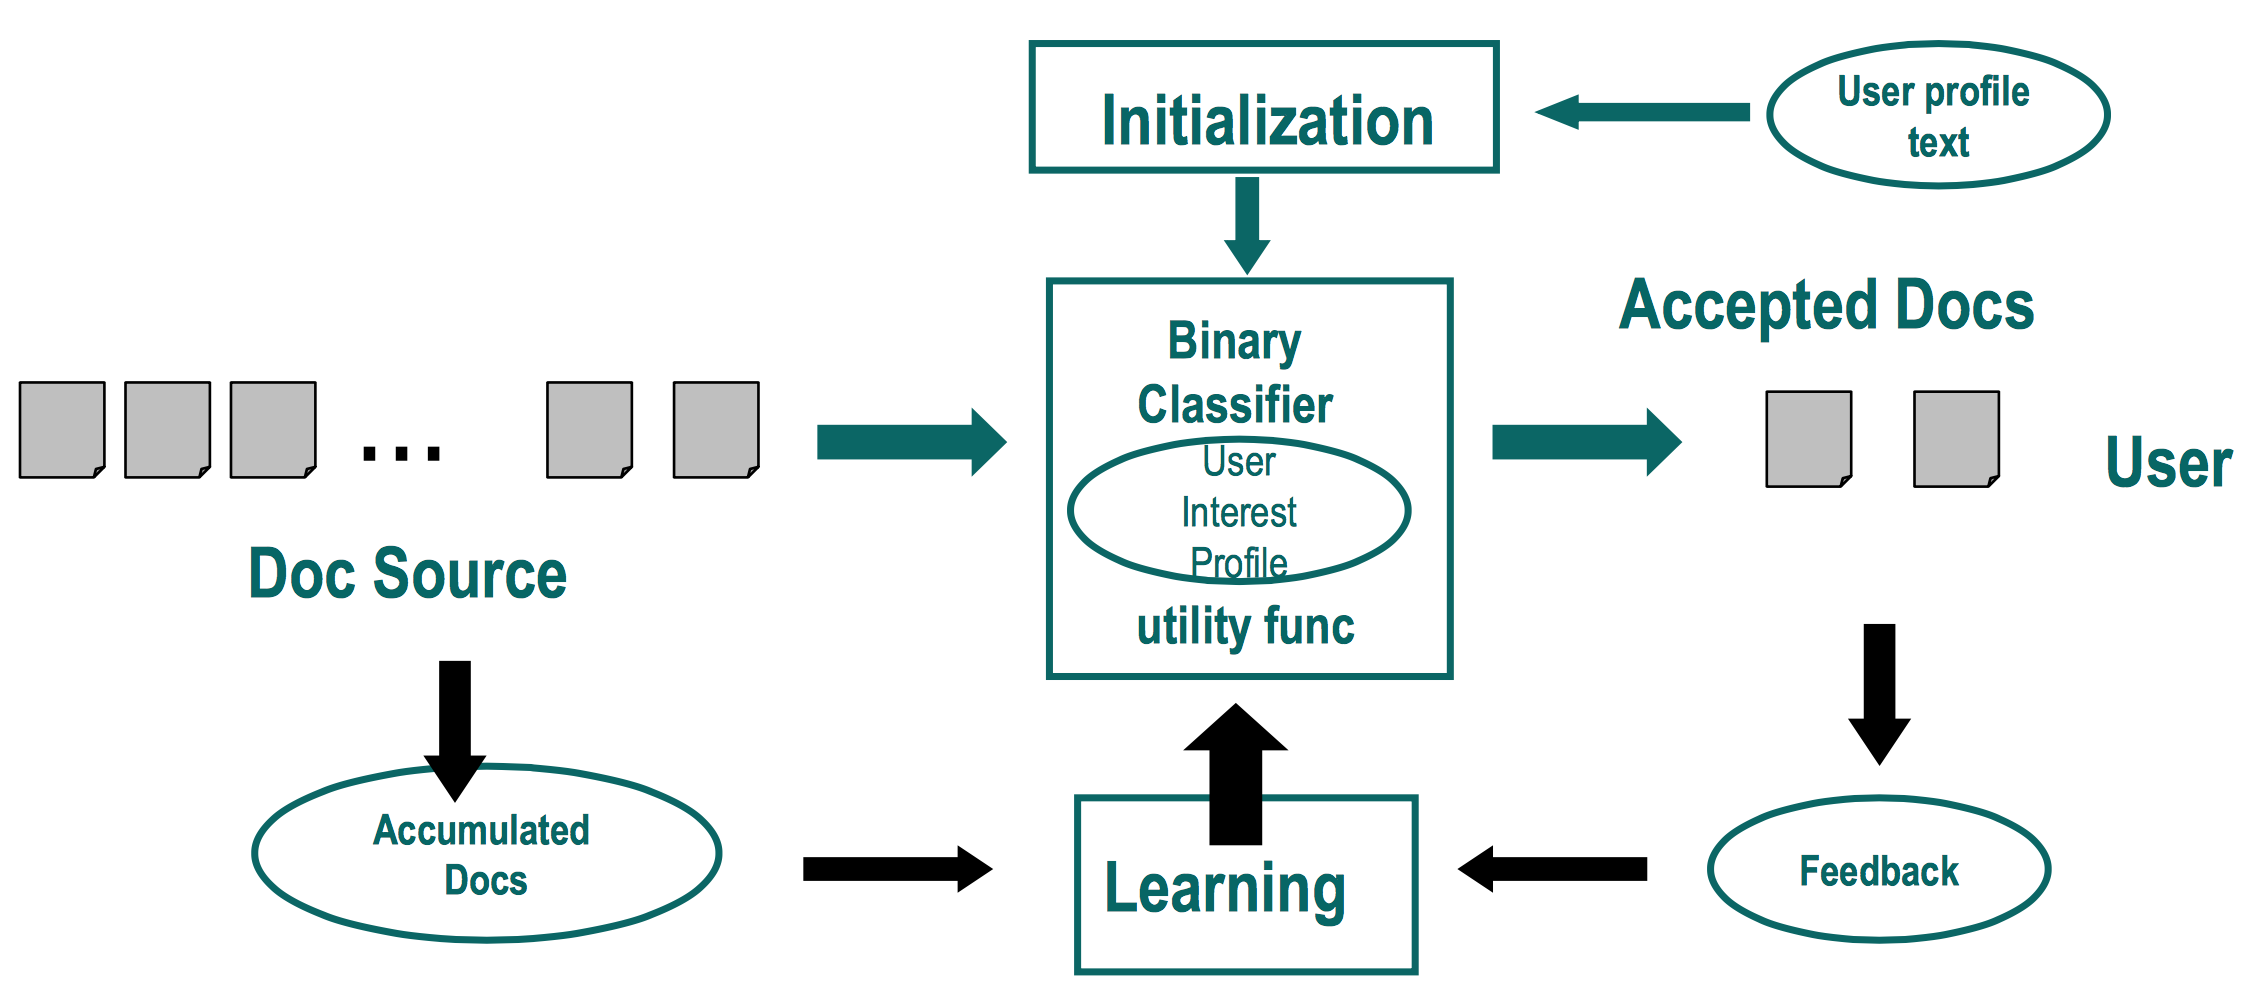
\includegraphics[width=0.9\linewidth]{content_based.png}
\end{figure}

Example of linear utility: 
\begin{equation*}
\text{Linear Utility} = 3 \times \#good - 2 \times \#bad
\end{equation*}


\subsubsection{Three Basic Problems in Content-Based Filtering}
\begin{itemize}
\item Making filtering decision (Binary classifier) 
\begin{itemize}
\item Doc text, profile text $\to$ yes/no
\end{itemize}

\item Initialization
\begin{itemize}
\item Initialize the filter based on only the profile text or very few examples
\end{itemize}

\item Learning from
\begin{itemize}
\item Limited relevance judgments (only on <<yes>> docs) – Accumulated documents
\end{itemize}

\item All trying to maximize the utility
\end{itemize}



\subsubsection{Extend a Retrieval System for Information Filtering}
Content-based recommender system can be built based on a search engine system:
\begin{itemize}
\item <<Reuse>> retrieval techniques to score documents
\item Use a score threshold for filtering decision
\item Learn to improve scoring with traditional feedback
\item New approaches to threshold setting and learning
\end{itemize}


\subsubsection{A General Vector-Space Approach}
\begin{figure}[H]
    \centering
    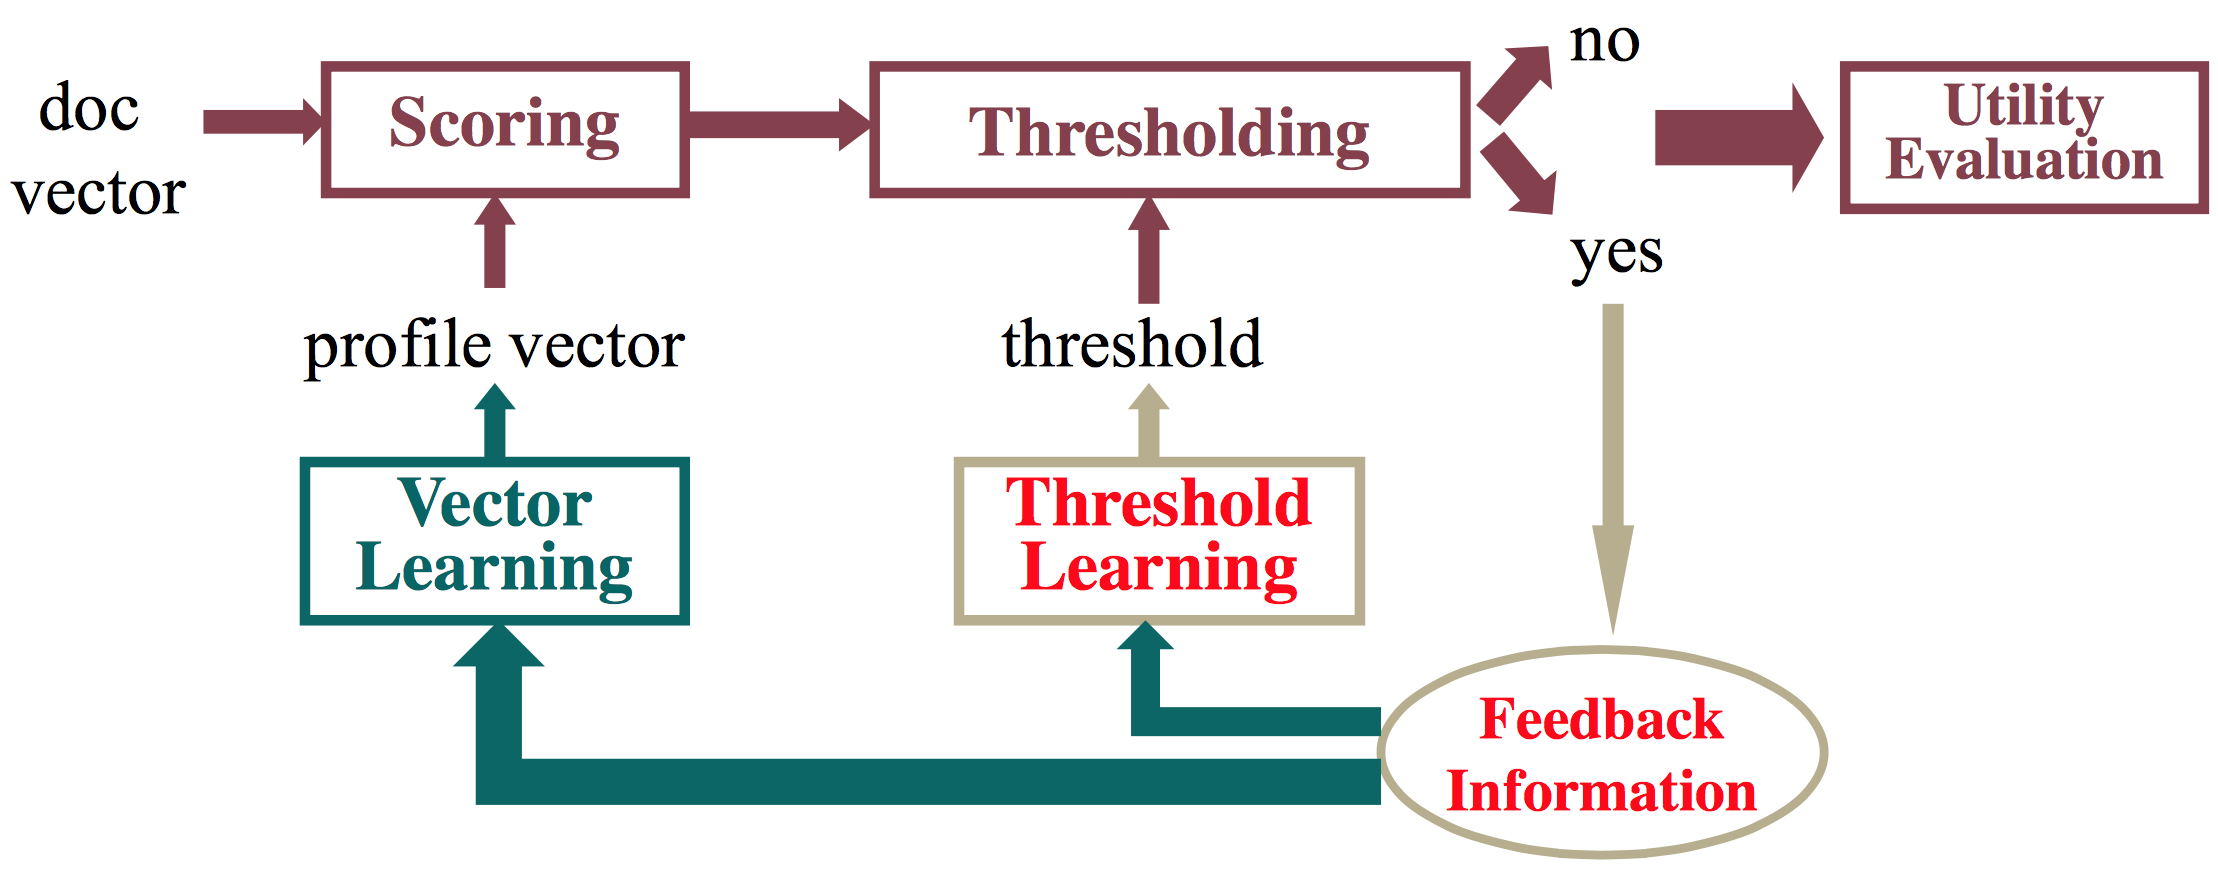
\includegraphics[width=0.9\linewidth]{content_based_vsm.png}
\end{figure}


\subsubsection{Difficulties in Threshold Learning}
\begin{itemize}
\item Censored data (judgments only available on delivered documents)
\item Little or none labeled data
\item Exploration vs. Exploitation
\end{itemize}


\subsubsection{Empirical Utility Optimization}
\begin{itemize}
\item Basic idea
\begin{itemize}
\item Compute the utility on the training data for each candidate score
threshold
\item Choose the threshold that gives the maximum utility on the training data set
\end{itemize}

\item Difficulty: Biased training sample!
\begin{itemize}
\item We can only get an upper bound for the true optimal threshold 
\item Could a discarded item be possibly interesting to the user?
\end{itemize}

\item Solution:
\begin{itemize}
\item Heuristic adjustment (lowering) of threshold
\end{itemize}
\end{itemize}


\subsubsection{Beta-Gamma Threshold Learning}

\begin{figure}[H]
    \centering
    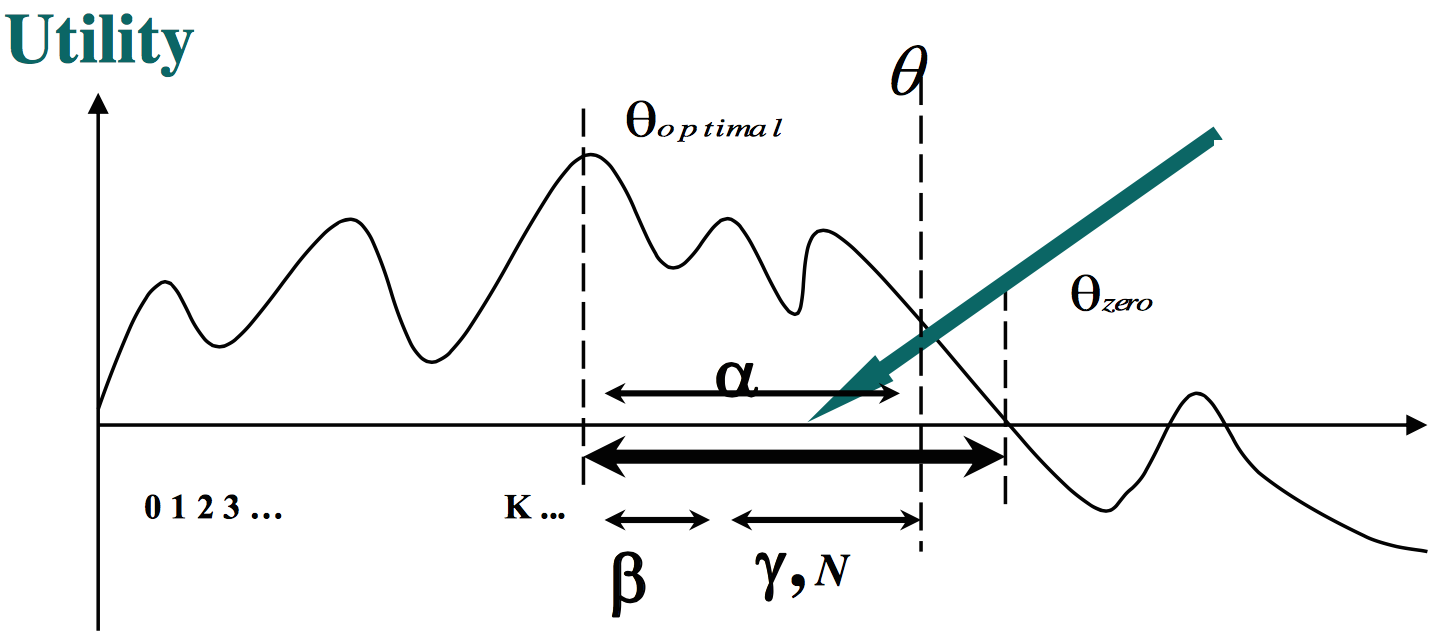
\includegraphics[width=0.7\linewidth]{beta_gamma.png}
\end{figure}

Encourage exploration of threshold up to $\theta_{zero}$:
\begin{equation*}
\theta = \alpha \times \theta_{zero} + (1-\alpha) \times \theta_{optimal}
\end{equation*}

The more examples, the less exploration (closer to $\theta_{optimal}$):
\begin{equation*}
\alpha = \beta + (1-\beta) \times e^{-N\gamma}, \text{ where }\beta,\gamma \in [0, 1]
\end{equation*}

\begin{itemize}
\item Pros:
\begin{itemize}
\item Explicitly addresses exploration-exploitation tradeoff (<<Safe>>
exploration)
\item Arbitrary utility (with appropriate lower bound)
\item Empirically effective
\end{itemize}

\item Cons:
\begin{itemize}
\item Purely heuristic
\item Zero utility lower bound often too conservative
\end{itemize}
\end{itemize}



%---------------------------------------------
\subsection{Collaborative Filtering}

\subsubsection{What is Collaborative Filtering (CF)?}
\begin{itemize}
\item Making filtering decisions for an individual user based on the judgments of other users
\item Inferring individual’s interest/preferences from that of other similar users
\item User similarity can be judged based on their similarity in preferences on a common set of items
\end{itemize}

CF assumptions
\begin{itemize}
\item Users with the same interest will have similar preferences
\item Users with similar preferences probably share the same interest
\item Sufficiently large number of user preferences are available (if not, there will be a <<cold start>> problem)
\end{itemize}


\newpage
\subsubsection{Memory-based Approaches to Collaboration Filtering Problem}

\begin{multicols}{2}

\begin{figure}[H]
    \centering
    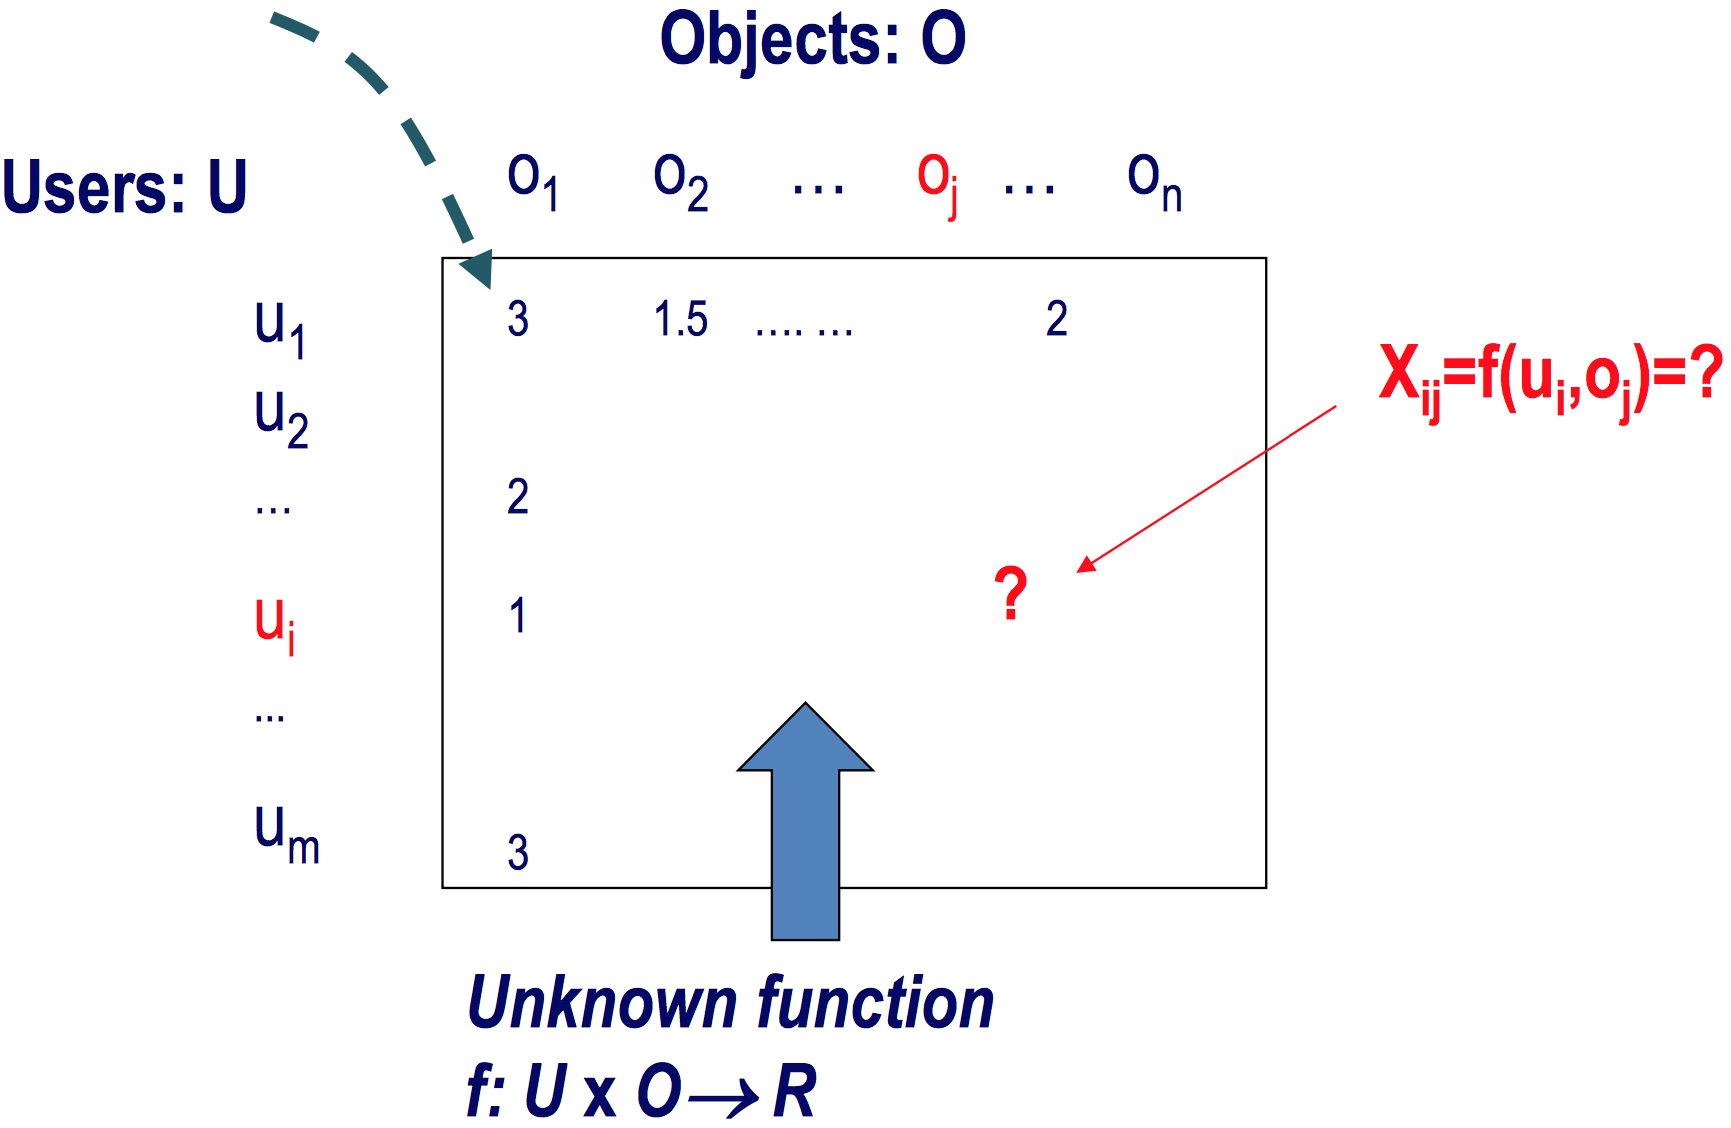
\includegraphics[width=\linewidth]{collaborative_problem.png}
\end{figure}

\columnbreak

\begin{itemize}
\item Assume we have $m$ users ($u_i$) and $n$ objects $o_j$
\item $x_{ij}$: rating of object $o_j$ by user $u_i$
\item $n_i$: average rating of all objects by user $u_i$ 
\item Normalized ratings: $v_{ij} = x_{ij} - n_i$
\end{itemize}
\end{multicols}

Prediction of rating of object $o_j$ by user $u_a$:
\begin{equation*}
\hat{v_{aj}} = \frac{\sum\limits_{i=1}^m v_{a,i} v_{ij}}{\sum\limits_{i=1}^m v_{a,i}}, \;\hat{x_{aj}} = \hat{v_{aj}} + n_a
\end{equation*}



\subsubsection{User Similarity Measures}
\begin{itemize}
\item Pearson correlation
\begin{equation*}
w_p(a, j) = \frac{\sum_j (x_{aj} - n_a)(x_{ij} - n_i)}{\sqrt{\sum_j (x_{aj} - n_a)^2 \sum_j(x_{ij} - n_i)^2}}
\end{equation*}

\item Cosine measure
\begin{equation*}
w_c(a, j) = \frac{\sum_j x_{aj} x_{ij}}{\sqrt{\sum_j x_{aj}^2 \sum_j x_{ij}^2}}
\end{equation*}
\end{itemize}


\subsubsection{Improving User Similarity Measures}
\begin{itemize}
\item Dealing with missing values: set to default ratings
\begin{itemize}
\item average ratings
\item iterate unknown ratings calculations followed by similarity measure calculation
\end{itemize}

\item Inverse User Frequency (IUF): similar to IDF
\end{itemize}



\subsubsection{Summary}
\begin{itemize}
\item Filtering/Recommendation is <<easy>>
\begin{itemize}
\item The user’s expectation is low
\item Any recommendation is better than none
\end{itemize}

\item Filtering is <<hard>>
\begin{itemize}
\item Must make a binary decision, though ranking is also possible
\item Data sparseness (limited feedback information)
\item <<Cold start>> (little information about users at the beginning)
\end{itemize}
\end{itemize}



\subsubsection{Recommended reading}
\begin{itemize}
\item Francesco Ricci, Lior Rokach, Bracha Shapira, Paul B. Kantor. \href{http://www.cs.bme.hu/nagyadat/Recommender_systems_handbook.pdf}{<<Recommender Systems Handbook>>}. Springer 2011.
\end{itemize}

%\newpage
\section{Course Summary}

\subsection{Recommended reading}
\begin{itemize}
\item \href{http://www.morganclaypool.com/page/ForthcomingSynthesisLectures}{Synthesis Digital Library} has many excellent short books/long tutorials on relevant topics
\begin{itemize}
\item \href{http://www.morganclaypool.com/toc/icr/1/1}{Information Concepts, Retrieval and Services}
\item \href{http://www.morganclaypool.com/toc/hlt/1/1}{Human Language Technology}
\item \href{http://www.morganclaypool.com/toc/aim/1/1}{Artificial Intelligence \& Machine Learning}
\end{itemize}

\item Journals: ACM TOIS, IRJ, IPM, ...
\item Conferences: SIGIR, CIKM, ECIR, WSDM, WWW, KDD, ACL, ...
\item \href{http://timan.cs.uiuc.edu/resources}{More info}
\item \href{http://searchuserinterfaces.com/}{Search User Interface}, by Marti Hearst, Cambridge University Press, 2009
\end{itemize}


\subsection{Main Techniques for Harnessing Big Text Data: Text Retrieval + Text Mining}
\begin{figure}[H]
    \centering
    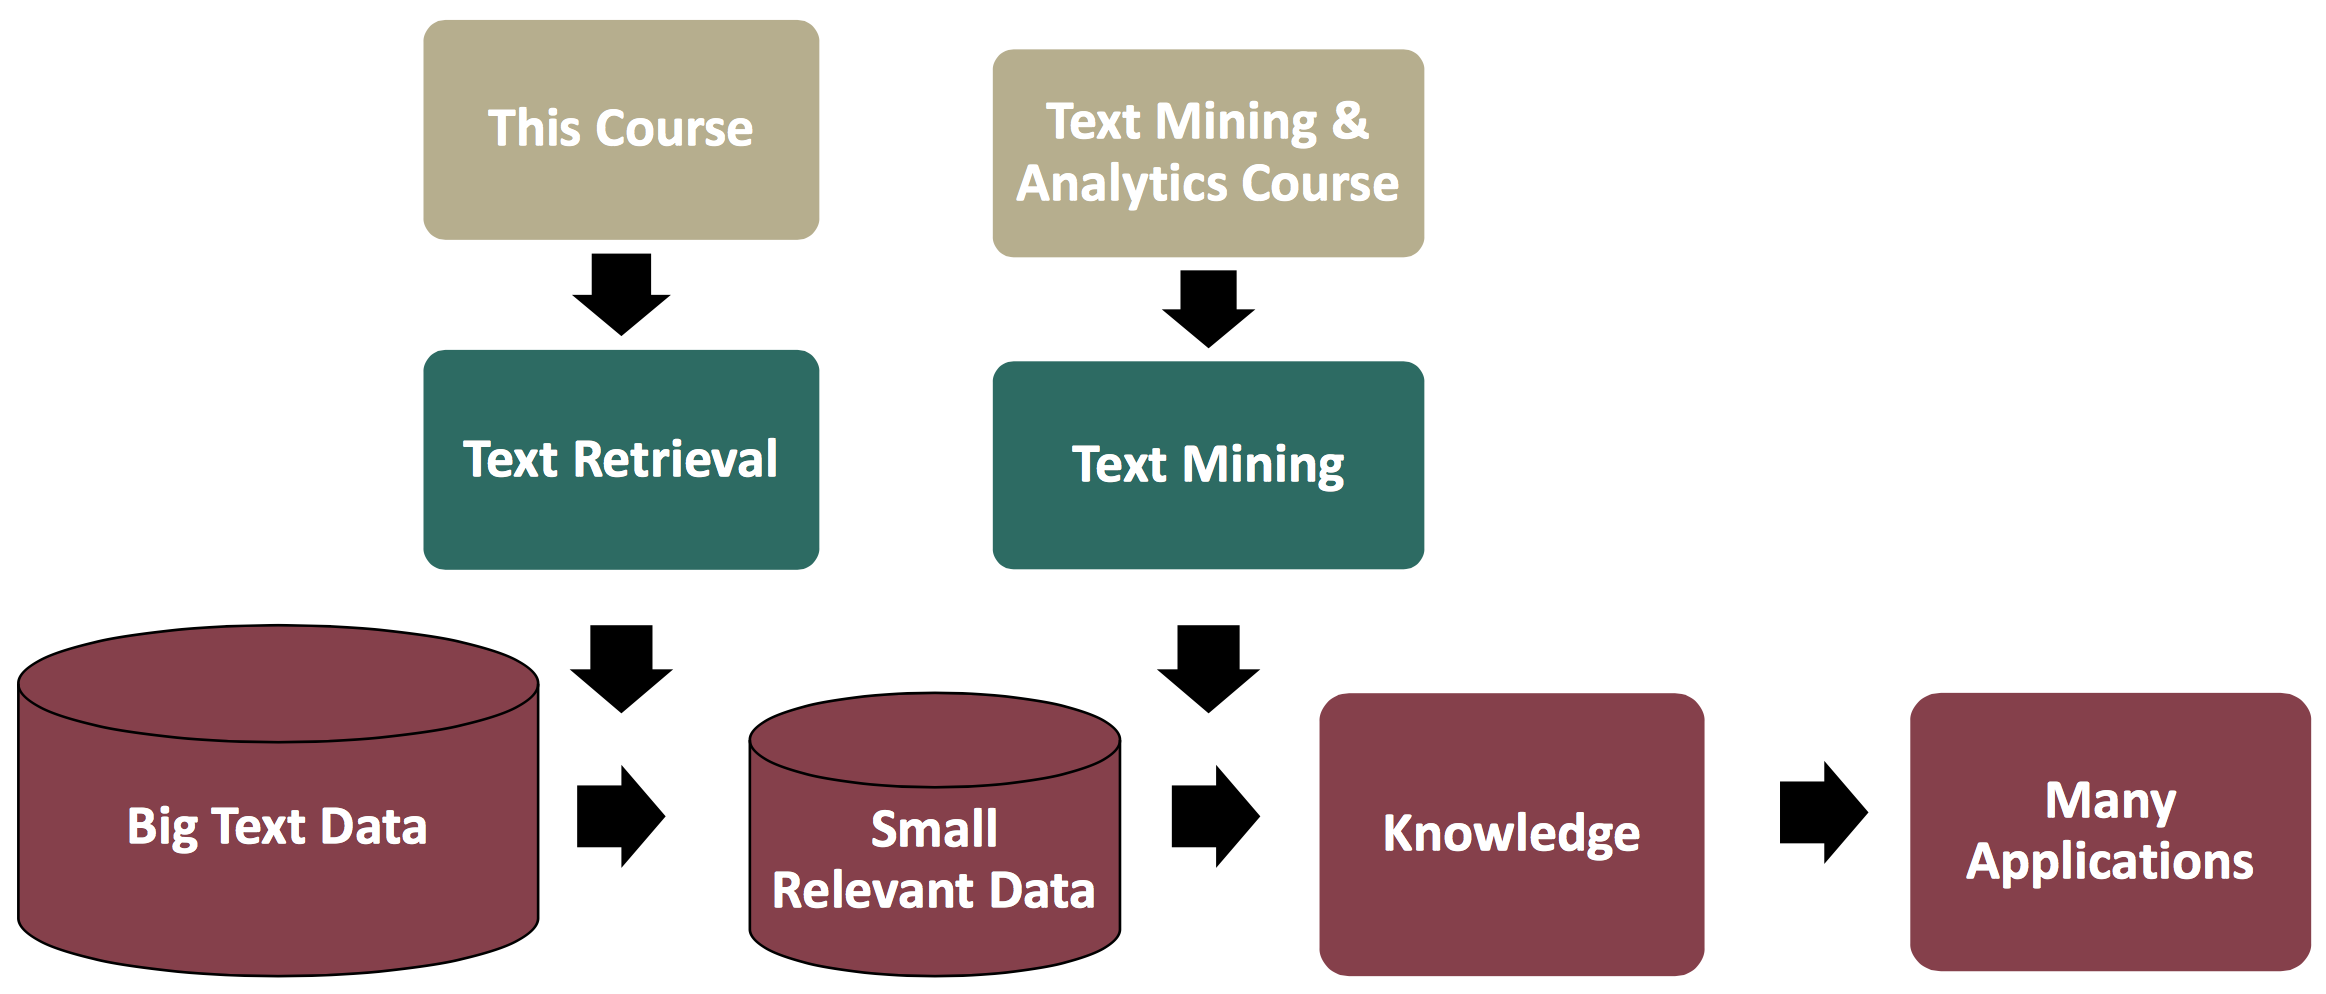
\includegraphics[width=0.9\linewidth]{big_text_data.png}
\end{figure}
%\input{lecture13.tex}

\end{document}
